%\VignetteIndexEntry{ODRF}
%\VignetteKeywords{CART, oblique decision tree, random forest, projection pursuit, R}
%\VignettePackage{ODRF}
%\VignetteEncoding{UTF-8}
%VignetteDepends{}
%paste0(getwd(),"/vignettes/ODRF-knitr.Rnw")

\documentclass[nojss]{jss}

%% -- LaTeX packages and custom commands ---------------------------------------

%% recommended packages
\usepackage{orcidlink,thumbpdf,lmodern}
%my packages
%\usepackage[ruled,linesnumbered]{algorithm2e}
\usepackage{subfig}
\usepackage{booktabs}
\usepackage{amsmath}
\usepackage{amssymb}
\usepackage{tikz}
\usetikzlibrary{shapes,arrows}
\tikzstyle{process} = [rectangle,draw=black!70,fill=white!30,rounded corners]
\tikzstyle{arrow} = [color=black,thick]


%% another package (only for this demo article)
\usepackage{framed}

%% new custom commands
\newcommand{\class}[1]{`\code{#1}'}
\newcommand{\fct}[1]{\code{#1()}}

%my commands
\numberwithin{equation}{section}
\DeclareMathOperator*{\argmin}{arg\,min}
\DeclareMathOperator*{\argmax}{arg\,max}
\def\E{{\mathbf E}}
\def\P{{\mathbf P}}
\def\x{{\bf x}}
\def\D{{\mathcal D}}
\def\O{{\mathcal O}}
\def\R{{\mathbb R}}
\def\S{{\cal S}}
\def\L{{\cal L}}
\def\B{{\mathbb{B}}}
\def\A{{\small\mathcal{A}}}
\def\C{{\small\mathcal{C}}}
\def\I{\mbox{I}}
\def\red{\color{black}}
\def\ind{{\perp \hspace{-0.2cm} \perp}}

%% For Sweave-based articles about R packages:
%% need no \usepackage{Sweave}
%TRUE}%

%% -- Article metainformation (author, title, ...) -----------------------------

%% - \author{} with primary affiliation (and optionally ORCID link)
%% - \Plainauthor{} without affiliations
%% - Separate authors by \And or \AND (in \author) or by comma (in \Plainauthor).
%% - \AND starts a new line, \And does not.
%~\orcidlink{0000-0003-0918-3766}
\author{Yu Liu\\National University of Singapore
   \And Yingcun Xia\\National University of Singapore}
\Plainauthor{Yu Liu, Yingcun Xia}

%% - \title{} in title case
%% - \Plaintitle{} without LaTeX markup (if any)
%% - \Shorttitle{} with LaTeX markup (if any), used as running title
\title{\pkg{ODRF}: An \proglang{R} Package for Oblique Decision Random Forest}
\Plaintitle{Oblique Decision Random Forest for Classification and Regression}
\Shorttitle{The \pkg{ODRF} \proglang{R} Package}

%% - \Abstract{} almost as usual
\Abstract{
%	\emph{CART} and Random Forest (\emph{RF}) have been widely used for data analysis, including prediction and classification. The use of linear combinations of predictors as a splitting variable is one of the most popular improvements to \emph{CART}. The method became known as the oblique decision tree (\emph{ODT}) and ODT-based random forests (\emph{ODRF}). There have been many related research achievements in theory, however, a complete and efficient package is still not available in computation. Therefore, to fill the current gap, we developed \pkg{ODRF} \proglang{R} package for prediction and classification, and provided online structure learning algorithms for \code{ODT} and \code{ODRF}. The main computational part of \code{ODT} is executed using \pkg{Rcpp} package and \code{ODRF} uses parallel computation, which significantly improves the computational efficiency. In the numerical experiments, \code{ODT} and \code{ODRF} are compared with other decision trees and forests, respectively, and the experimental results are shown that \code{ODT} and \code{ODRF}  has a noticeable overall improvement.
	
\emph{CART} and Random Forest (\emph{RF}) are arguably the most popular methods in statistical data analysis and forecasting. The use of linear combinations of predictors as splitting variables is one of the important extensions of \emph{CART} and is known as Oblique Decision Trees (\emph{ODT}) and ODT-based Random Forests (\emph{ODRF}). Recent studies have also shown the theoretical advantages of \emph{ODT} and \emph{ODRF} over \emph{CART} and \emph{RF}. However, there is still no integrated and efficient software package that can demonstrate the numerical advantages of \emph{ODT} and \emph{ODRF}. To fill this gap, we developed an \pkg{ODRF} \proglang{R} package for both \code{ODT} and \code{ODRF}, and provided online structure learning algorithms. The main computational part of \code{ODT} is executed using the \pkg{Rcpp} package, and \code{ODRF} allows parallel computation. Through numerical experiments, our package was compared with other packages for decision trees and forests, showing a clear overall improvement.%, and provided online structure learning algorithms
	
	%Abstract: %As a remedy  for the deficiencies of the standard classification regression tree (CART), \cite{breiman1984classification} suggested using linear combinations of predictors as splitting variables. The method became known as the oblique decision tree (ODT) and has received much attention. ODT has better performance than CART, requiring fewer splits and therefore smaller trees than CART; the linear combination also makes ODT easy to interpret in data analysis. In this paper, we further show that ODT is also a remedy for the statistical consistency problem that CART cannot solve, in that ODT is consistent for general regression functions or classification problems. We also study the consistency of ODT-based random forests, hereafter referred to as ODRF. We introduce an algorithm for ODRF, and show through extensive experiments that ODRF generally yields better performance than existing decision forests.
	
%The oblique decision tree is a popular choice in the machine learning domain for improving the performance of traditional decision tree algorithms. In contrast to the traditional decision tree, which uses an axis-parallel split point to determine whether a data point should be assigned to the left or right branch of a decision tree, the oblique decision tree uses a hyper-plane based on all data point features.
%Numerous works in the machine learning domain have shown that oblique decision trees can achieve exceptional performance in a wide range of domains. However, there is still a lack of a package that has implemented oblique decision tree algorithms, which stymies the development of this domain. As a result, the goal of this project is to solve this problem by implementing some well-known algorithms in this domain. We hope that by doing so, these algorithms will serve as a baseline for machine learning practitioners to compare newly designed algorithms to existing algorithms.


%\emph{CART} and Random Forest (\emph{RF}) have been widely used for data analysis, including prediction and classification. The use of linear combinations of predictors as a splitting variable is one of the most popular improvements to \emph{CART}. The method became known as the oblique decision tree (\emph{ODT}) and ODT-based random forests (\emph{ODRF}). There have been many related research achievements in theory, however, a complete and efficient package is still not available in computation. Therefore, to fill the current gap, we developed \pkg{ODRF} \proglang{R} package for prediction and classification, and provided online structure learning algorithms for \code{ODT} and \code{ODRF}. The main computational part of \code{ODT} is executed using \pkg{Rcpp} package and \code{ODRF} uses parallel computation, which significantly improves the computational efficiency. In the numerical experiments, \code{ODT} and \code{ODRF} are compared with other decision trees and forests, respectively, and the experimental results are shown that \code{ODT} and \code{ODRF}  has a noticeable overall improvement.

	%Abstract: %As a remedy  for the deficiencies of the standard classification regression tree (CART), \cite{breiman1984classification} suggested using linear combinations of predictors as splitting variables. The method became known as the oblique decision tree (ODT) and has received much attention. ODT has better performance than CART, requiring fewer splits and therefore smaller trees than CART; the linear combination also makes ODT easy to interpret in data analysis. In this paper, we further show that ODT is also a remedy for the statistical consistency problem that CART cannot solve, in that ODT is consistent for general regression functions or classification problems. We also study the consistency of ODT-based random forests, hereafter referred to as ODRF. We introduce an algorithm for ODRF, and show through extensive experiments that ODRF generally yields better performance than existing decision forests.
	
	%The classification and regression tree (CART) and Random Forest (RF) are arguably the most popular pair of statistical learning methods. However, their statistical consistency can only be proved under very restrictive assumption on the underlying regression function. As an extension of the standard CART, \cite{breiman1984classification} suggested using linear combinations of predictors as splitting variables. The method became known as the oblique decision tree (ODT) and has received lots of attention. ODT tends to perform better than CART and requires fewer partitions. In this paper, we further show that ODT is consistent for very general regression functions as long as they are continuous. We also prove the consistency of ODT-based random forests (ODRF) that uses either fixed-size or random-size subset of features in the features bagging, the latter of which is also guaranteed to be consistent for general regression functions, but the former is consistent only for functions with specific structures.  After refining the existing computer packages according to the established theory, our numerical experiments also show that ODRF has a noticeable overall improvement over RF and other decision forests.
	%The classification and regression tree (CART) and Random Forest (RF) are arguably the most popular pair of statistical learning methods. However, their statistical consistency can only be proved under very restrictive assumption on the underlying regression function. As an extension of standard CART, the oblique decision tree (ODT), which uses linear combinations of predictors as partitioning variables, has received much attention. ODT tends to perform numerically better than CART and requires fewer partitions. In this paper, we further show that ODT is consistent for very general regression functions as long as they are continuous. We also prove the consistency of ODT-based random forests (ODRF) that uses either fixed-size or random-size subset of features in the features bagging, the latter of which is also guaranteed to be consistent for general regression functions, and the former is consistent only for functions with specific structures.  After refining the existing computer packages according to the established theory, our numerical experiments also show that ODRF has a noticeable overall improvement over RF and other decision forests.
	
	% letter:
	%CART and random forests (RF) have been a hot research topic in statistics and machine learning for many years. Recently, Scornet et al. (2015, AOS) have made a milestone progress in statistical consistency, bringing a new phase of research in related topics. However, the consistency further confirms the theoretical weaknesses of standard CART and RF. This motivates us to study the consistency of the oblique decision trees (ODT), a generalization of CART.
	%In this paper, we establish a complete theory for ODT and introduce new feature bagging methods, resulting in new random forests. We also implement the new random forests and further demonstrate the numerical advantages of ODT and its random forests over the standard RF.
	%I would appreciate if you could consider publishing this paper in Bernoulli.
	
	%while the existing consistency result of RF is a corollary of our consistency results.
	
	%We present an algorithm for ODRF, and demonstrate through extensive experiments that ODRF generally yields better performance than existing decision forests.
	
	%\vspace{0.2cm}
	
	%CART and Random Forest (RF) have been widely used for data analysis, including prediction and classification. However, their statistical consistency can only be proved under very restrictive model assumptions. In addition to technical difficulties, their own limitations are another reason for the lack of consistency guarantees. This problem was already observed when CART was proposed by \cite{breiman1984classification}, who suggested using linear combinations of predictors as splitting variables as a remedy. This idea was later intensively studied, called Oblique Decision Tree (ODT), and has demonstrated better performance than CART or RF. This paper aims to provide the theory for ODT and ODT-based random forest (ODRF) to be consistent for general models without requiring strong assumptions. We also propose a way to build the linear combinations of randomly selected features as splitting variables to implement ODRF. Extensive experiments show that ODRF typically yields improved performance over existing decision forests.
	
  %This short article illustrates how to write a manuscript for the
 % \emph{Journal of Statistical Software} (JSS) using its {\LaTeX} style files.
 % Generally, we ask to follow JSS's style guide and FAQs precisely. Also,
 % it is recommended to keep the {\LaTeX} code as simple as possible,
 % i.e., avoid inclusion of packages/commands that are not necessary.
 % For outlining the typical structure of a JSS article some brief text snippets
 % are employed that have been inspired by \cite{Zeileis+Kleiber+Jackman:2008},
 % discussing count data regression in \proglang{R}. Editorial comments and
 % instructions are marked by vertical bars.
}

%% - \Keywords{} with LaTeX markup, at least one required
%% - \Plainkeywords{} without LaTeX markup (if necessary)
%% - Should be comma-separated and in sentence case.
\Keywords{CART, oblique decision tree, random forest, projection pursuit, \proglang{R}}
\Plainkeywords{CART, oblique decision tree, random forest, projection pursuit, R}

%% - \Address{} of at least one author
%% - May contain multiple affiliations for each author
%%   (in extra lines, separated by \emph{and}\\).
%% - May contain multiple authors for the same affiliation
%%   (in the same first line, separated by comma).
%%\Address{
%%  Achim Zeileis\\
%%  Journal of Statistical Software\\
%%  \emph{and}\\
%%  Department of Statistics\\
%%  Faculty of Economics and Statistics\\
%%  Universit\"at Innsbruck\\
%%  Universit\"atsstr.~15\\
%%  6020 Innsbruck, Austria\\
%%  E-mail: \email{Achim.Zeileis@R-project.org}\\
%%  URL: \url{https://www.zeileis.org/}
%%}

\Address{
  Yu Liu\\
  Department of Statistics and Data Science\\
  National University of Singapore, Singapore\\
  E-mail: \email{liuyuchina123@gmail.com}\\
  %URL: \url{https://www.zeileis.org/}

  Yingcun Xia\\
  Department of Statistics and Data Science\\
  National University of Singapore, Singapore\\
  E-mail: \email{staxyc@nus.edu.sg}\\
  %URL: \url{https://www.zeileis.org/}
}

\begin{document}

%% -- Introduction -------------------------------------------------------------

%% - In principle "as usual".
%% - But should typically have some discussion of both _software_ and _methods_.
%% - Use \proglang{}, \pkg{}, and \code{} markup throughout the manuscript.
%% - If such markup is in (sub)section titles, a plain text version has to be
%%   added as well.
%% - All software mentioned should be properly \cite-d.
%% - All abbreviations should be introduced.
%% - Unless the expansions of abbreviations are proper names (like "Journal
%%   of Statistical Software" above) they should be in sentence case (like
%%   "generalized linear models" below).

\section{Introduction} \label{sec:intro}

%\begin{leftbar}
%The introduction is in principle ``as usual''. However, it should usually embed
%both the implemented \emph{methods} and the \emph{software} into the respective
%relevant literature. For the latter both competing and complementary software
%should be discussed (within the same software environment and beyond), bringing
%out relative (dis)advantages. All software mentioned should be properly
%\verb|\cite{}|d. (See also Appendix~\ref{app:bibtex} for more details on
%\textsc{Bib}{\TeX}.)

%For writing about software JSS requires authors to use the markup
%\verb|\proglang{}| (programming languages and large programmable systems),
%\verb|\pkg{}| (software packages), \verb|\code{}| (functions, commands,
%arguments, etc.). If there is such markup in (sub)section titles (as above), a
%plain text version has to be provided in the {\LaTeX} command as well. Below we
%also illustrate how abbrevations should be introduced and citation commands can
%%\end{leftbar}


%The Classification and Regression Tree (CART) proposed by Professor Leo Brieman (1984) has attracted a great deal of attention from statisticians and data analysts from other disciplines. The method is widely used because it is easy to train and the resulting tree makes the analysis results visual and easy to interpret. On the other hand, attention has been paid to the algorithm and many improvements have been proposed.

%In practical studies, many of the problems we experience are always complex, and the relationship between individual features is usually nonlinear. Decision trees have an important advantage for handling heterogeneous data with ease when different features come from different sources , and are widely employed methods for classification and regression. This makes decision trees a popular “off-the-shelf” machine learning method that can be readily applied to any data without much tuning \citep{2014Learning}. Classification and regression trees (\emph{CART}) \cite{quinlan1987decision} and \emph{C4.5} \cite{quinlan1993program} are the most commonly used decision trees with different partition criteria.

%The Classification and Regression Tree (\emph{CART}) proposed by \cite{quinlan1987decision} has attracted a great deal of attention from statisticians and data analysts from other disciplines. The method is widely used because it is easy to train and the resulting tree makes the analysis results visual and easy to interpret. On the other hand, attention has been paid to the algorithm and many improvements have been proposed, including mainly Evolutionary Learning of Globally Optimal Classification and Regression Trees (\emph{EVT}) \cite{Grubinger2014ectree},  Conditional Inference Trees (\emph{CT}) \cite{hothorn2006unbiased}, Extremely randomized trees (\emph{ERT}) \cite{2006Extremely}, Model-Based Recursive Partitioning (\emph{MOB}) \cite{zeileis2015parties}, bayesian additive regression trees (\emph{BART}) \cite{maia2022gp} and generalized linear mixed-model trees (\emph{glmertree}) \cite{2020Generalized}. Over the last two decades, ensemble methods have risen to prominence as the stateof-the-art for general-purpose machine learning tasks. One of the most popular and consistently strong ensemble methods is Random Forests (\emph{RF}) \cite{breiman2001random}, which uses decision trees \emph{CART} as the base learners \citep{tomita2020sparse}. In addition, there are many decision tree based ensemble methods. For example, Conditional Random Forests (\emph{cforest}) \cite{hothorn2006unbiased}, Learning Nonlinear Functions Using Regularized Greedy Forest (\emph{RGF}) \cite{2014Learning}, Generalized Random Forest (\emph{GRF}) \cite{athey2019generalized} and extreme gradient boosting (\emph{XGB}) \cite{chen2016xgboost}.

The Classification and Regression Tree (CART) proposed by Professor Leo Brieman (1984) has attracted a great deal of attention from statisticians and data analysts of other disciplines. The method is widely used because it is easy to train and the resulting tree makes the analysis results visual and easy to interpret \citep{2014Learning}. On the other hand, much attention has been paid to the algorithm and many improvements have been proposed. Classification and regression trees  \cite[CART]{quinlan1987decision} and \emph{C4.5} \cite{quinlan1993program} are the most commonly used decision trees. There is a long list of other decision trees, including the Evolutionary Learning of Globally Optimal Classification and Regression Trees (\emph{EVT}) \cite{Grubinger2014ectree},  Conditional Inference Trees (\emph{CT}) \cite{hothorn2006unbiased}, Extremely randomized trees (\emph{ERT}) \cite{2006Extremely}, Model-Based Recursive Partitioning (\emph{MOB}) \cite{zeileis2015parties}, bayesian additive regression trees (\emph{BART}) \cite{maia2022gp} and generalized linear mixed-model trees (\emph{glmertree}) \cite{2020Generalized}.  The Random Forests \citep[RF]{breiman2001random}, which is an ensemble of CARTS by either feature bagging or boosting,   is arguably the most efficient machine method especially for the tabular data \cite{tabularDATA}. Again, there are many ensemble methods that based on different decision trees. For example, Conditional Random Forests (\emph{cforest}) \cite{hothorn2006unbiased}, Learning Nonlinear Functions Using Regularized Greedy Forest (\emph{RGF}) \cite{2014Learning}, Generalized Random Forest (\emph{GRF}) \cite{athey2019generalized} and extreme gradient boosting (\emph{XGB}) \cite{chen2016xgboost}.


One of the most appealing extensions to CART is the use of linear combinations of the predictors as splitting variables that is known as the Oblique Decision tree \cite{Heath93inductionof}. Recently, \cite{zhan2022consistency} proved the consistency of The Oblique Decision Tree (\emph{ODT}) and Its Random Forest for very general regression functions as long as they are continuous, while CART or RF are consistency mainly for regressions with special structures such as additive structure.  Again, ensemle can be made based on ODT resulting the Oblique-type Random Forests, including Random Rotation Random Forest (\emph{RR-RF}) of \cite{blaser2016random}, Random Projection Forests (\emph{RPFs}) of \cite{lee2015fast} and Sparse Projection Oblique Random Forests (\emph{SPORF}) of \cite{tomita2020sparse}. Another type is the model-based oblique decision forest,  including mainly Canonical Correlation Forests (\emph{CCF}) with classic correlation analysis \cite{rainforth2015canonical},  projection pursuit forest (\emph{PPF}) with linear discriminant analysis \cite{silva2021projection}, oblique random forests (\emph{ORF}) with ridge regression \cite{menze2011oblique}, oblique random survival forests (\emph{ORSF}) \cite{jaeger2022accelerated} and Heterogeneous oblique random forest (\emph{HORF}) \cite{katuwal2020heterogeneous}.

%However, all the ensemble methods mentioned above are ensembles of "axis-aligned" decision trees, restricting the ensemble decision surfaces to be piecewise axis-aligned, even when there is little evidence for this in the data. To address this, \cite{breiman2001random} also proposed and characterized Forest-RC (\emph{F-RC}), which splits on linear combinations of coordinates rather than individual coordinates. These so-called “oblique” ensembles include the axis-aligned ensembles as a special case, and therefore have better numerical performance and requires fewer partitions. Therefore, it has also aroused widely interest and numerous other oblique decision forest methods have been proposed. There are two main types: one is the random ensemble forest similar to \emph{F-RC}, including mainly Random Rotation Random Forest (\emph{RR-RF}) of \cite{blaser2016random}, Random Projection Forests (\emph{RPFs}) of \cite{lee2015fast} and Sparse Projection Oblique Random Forests (\emph{SPORF}) of \cite{tomita2020sparse}; Another type is the model-based oblique decision forest,  including mainly Canonical Correlation Forests (\emph{CCF}) with classic correlation analysis \cite{rainforth2015canonical},  projection pursuit forest (\emph{PPforest}) with linear discriminant analysis \cite{silva2021projection}, oblique random forests (\emph{obliqueRF}) with ridge regression \cite{menze2011oblique}, oblique random survival forests (\emph{ORSF}) \cite{jaeger2022accelerated} and Heterogeneous oblique random forest (\emph{HORF})\cite{katuwal2020heterogeneous}. \cite{zhan2022consistency} proof the consistency of The Oblique Decision Tree (\emph{ODT}) and Its Random Forest. we further show that \emph{ODT} is consistent for very general regression functions as long as they are continuous. we also prove the consistency of ODT-based random forests (\emph{ODRF}) that uses either fixed-size or random-size subset of features in the features bagging. \cite{biau2008consistency} proposed a binary classification problem for which Breiman's \emph{RF} is inconsistent. \emph{ODRF} and other oblique methods are empirically more consistent on at least some settings on which \emph{RF} is neither empirically or theoretically consistent.

Although the theoretical advantages of oblique decision trees and their random forests have been well understood, the existing packages implementing those extensions only show their better numerical performance in some special cases, and thus not commonly received and have not got as much as popularity as they deserve. As a consequence, the conventional CART and RF are still the most commonly used packages.    The main difficulty in implementing \emph{ODT} or \emph{ODRF} is the estimation of the coefficient, $ \theta $, for the linear combinations, which is also one of the main differences amongst all the existing packages. The estimation methods  of $ \theta $ include random projection, logistic regression, dimension reduction and many others. For example, the functions \fct{RerF} in \pkg{rerf} package \cite{tomita2020sparse} use random projections, the functions \fct{baggtree} in \pkg{PPforest} package \cite{silva2021projection} uses  \code{"LDA"} model to estimate the projection directions, and they also provide the  \code{"PDA"}, \code{"GINI"} and  \code{"ENTROPY"} models in parameter \code{PPmethod}; the functions \fct{obliqueRF} in \pkg{obliqueRF} package \cite{menze2011oblique} uses \code{"ridge"} for fast ridge regression using SVD (default), \code{"pls"} for partial least squares regression, \code{"svm"} for a linear support vector machine, \code{"log"} for logistic regression and \code{"rnd"} for a random hyperplane in parameter \code{training\_method}. %However, all existing \proglang{R} packages can only be used for classification and are very time consuming to compute.
Some of the \proglang{R} packages have been taken off from the Comprehensive \proglang{R} Archive Network (CRAN) at \url{https://CRAN.R-project.org/} by \citep{R} due to some problems and have not been modified.


We refine the existing computer  \proglang{R} \citep{R} packages according to the established theory in the article of \cite{zhan2022consistency}. Our package, called \pkg{ODRF}, is modified from several existing \proglang{R} packages.
In \pkg{ODRF}, the projection pursuit regression function is used to find $ \theta $ for each set of $ q $ predictors, but other options are also provided in the package. Of course many \proglang{R}  packages have been developed  to implement \emph{ODT} and \emph{ODRF}.
Our \pkg{ODRF} \proglang{R} package can be used for classification and regression, and the computational time consumption and estimation accuracy are better than the competitive \proglang{R} package. Comparing with , our advantages
\begin{itemize}

\item Both the tree and forests of \pkg{ODRF} have better overall accuracy than existing trees and forests, including traditional CART and RF, in both classification and regression prediction, respectively.

%\item ODT of \pkg{ODRF} can plot the generated tree for users to analysis the data statistically.

\item \pkg{ODRF} can be used for both classification and regression, while most existing packages of oblique-type trees or forests only make classification.

\item \pkg{ODRF} allows users to define their own functions to find the projections of at each node, which is essential to the performance of the forests.

\item \pkg{ODRF} also applies to streaming data and continuously improves the existing tree.

\end{itemize}


The remainder of this paper is organized as follows: Section \ref{sec:models}, shows the model or algorithm details of the main functions in the \pkg{ODRF} package, so that the user has a clear understanding of the relevant principles. In Section \ref{sec:functions}, Introduce the usage of \pkg{ODRF} package. In Section {sec:examples}, use the \pkg{ODRF} package to compare the predictive effects in classification and regression with other \proglang{R} packages and showcase the specific application of the ODRF package in practice by two data sets with continuous and categorical responses. The summary in Section \ref{sec:summary} gives concluding remarks about the implementation and the performance of the new algorithm; further technical details are presented in the appendix.

	%We compare two different random rotation ensemble oblique tree methods, the first one is Blaser and Fryzlewicz\cite{blaser2016random} proposed the Random Rotation Random Forest (RotRF) method, which uniformly randomly rotates the data prior to inducing each tree. Trees are then learned via the typical axis-aligned procedure on the rotated data. The second one is Tomita et al.\cite{tomita2020sparse} proposed Sparse Projection Oblique Randomer Forests (SPORF) use the procedure laid out in Blaser and Fryzlewicz\cite{blaser2016random} based on a QR decomposition of independent draws from a unit Gaussian. Note that, SPORF unlike RotRF, the random rotation in SPORF is carried out at separately each node, as opposed to using a single rotation for the whole tree. SPORF unlike also F-RC of Breiman\cite{breiman2001random}, one key difference between the random projection distribution of SPORF and F-RC is that F-RC requires that a hyperparameter be specified to fix the sparsity of the sampled univariate projections (i.e., individual linear combinations). SPORF is more robust to the choice of sparsity level than F-RC\cite{tomita2020sparse}.
	
%Extremely randomized trees
%Generalized linear mixed-model (GLMM) trees
% Extremely randomized trees (extraTrees)
%An Introduction to Recursive Partitioning Using the RPART Routines
%Partykit: a modular toolkit for recursive partytioning in R
%Package ‘logicDT???
%Conditional Inference Trees


%% -- Manuscript ---------------------------------------------------------------

%% - In principle "as usual" again.
%% - When using equations (e.g., {equation}, {eqnarray}, {align}, etc.
%%   avoid empty lines before and after the equation (which would signal a new
%%   paragraph.
%% - When describing longer chunks of code that are _not_ meant for execution
%%   (e.g., a function synopsis or list of arguments), the environment {Code}
%%   is recommended. Alternatively, a plain {verbatim} can also be used.
%%   (For executed code see the next section.)


%\section{Models and software} \label{sec:models}
%\section{Models} \label{sec:models}
%\subsection{Basic algorithm}
%\subsection{program developments}
\section{The underlying algorithm} \label{sec:models}
%\subsection{Basic algorithm}
%\subsection{program developments}


The main step in the ODT or ODRF is the estimation and selection of the lienar combinations. Although many methods have been proposed, we find the projection pursuit regression is still the most efficient and is used. Suppose the $ Y_1, ..., Y_q $ are the responses. Typically, if $ q = 1$ then  $ Y_1 $ is continuous response or two classes denoted by 0 and 1; if $ q > 1$, it means there are $ q+1 $ classes denoted by $ (0, ..., 1, ...0)    $


\begin{figure}[t!]
    \centering
    %\includegraphics{}
   % \resizebox{8cm}{!}{%
 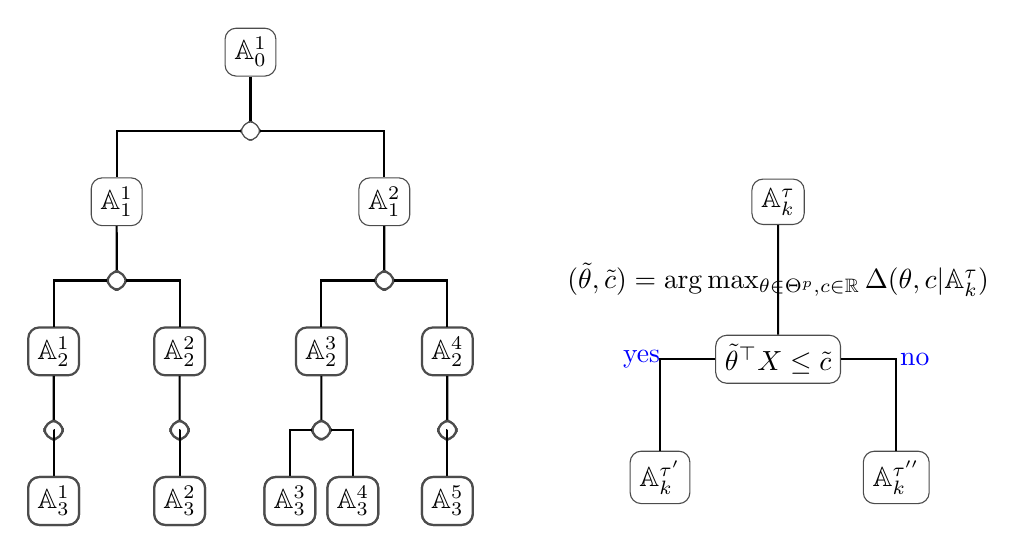
\begin{tikzpicture}[node distance=1cm,scale=0.6,
 	edge from parent/.style={black,thick,draw},	
 	edge from parent path={(\tikzparentnode) -| (\tikzchildnode)}]
 	
 	%ODT1
 	\node (S01) [process] {$\mathbb{A}_0^1$};
 	\node (N01) [process,below of=S01] {};
 	\draw [arrow] (S01) -- (N01);
 	\node (N01) [process,below of=S01] {}
 	child {
 		node (S11) [process,xshift=1cm] {$\mathbb{A}_1^1$};
 		\node (N11) [process,below of=S11] {};
 		\draw [arrow] (S11) -- (N11);
 		\node (N11) [process,below of=S11] {}
 		child {
 			node (S21) [process, xshift=1cm ] {$\mathbb{A}_2^1$};
 			\node (N21) [process,below of=S21] {};
 			\draw [arrow] (S21) -- (N21);
 			\node (N21) [process,below of=S21] {}
 			child {
 				node (S31) [process] {$\mathbb{A}_3^1$};
 				%\draw [arrow] (S33) -- ++(0,-1.5);
 				\node (S31) [process] {$\mathbb{A}_3^1$}
 			}
 			%			child {
 				%				node (S31) [process] {$\mathbb{A}_3^1$};
 				%				\node (S31) [process] {$\mathbb{A}_3^1$}
 				%			}
 			%			child [missing] {}
 			%			child {
 				%				node (S32) [process] {$\mathbb{A}_3^2$};
 				%				\node (S32) [process] {$\mathbb{A}_3^2$}
 				%			}
 		}
 		child [missing] {}	
 		child [missing] {}
 		child [missing] {}
 		child {
 			node (S22) [process,xshift=-1cm] {$\mathbb{A}_2^2$};
 			\node (N22) [process,below of=S22] {};
 			\draw [arrow] (S22) -- (N22);
 			\node (N22) [process,below of=S22] {}
 			child {
 				node (S33) [process] {$\mathbb{A}_3^2$};
 				%\draw [arrow] (S33) -- ++(0,-1.5);
 				\node (S33) [process] {$\mathbb{A}_3^2$}
 			}
 		}
 	}		
 	child [missing] {}	
 	child [missing] {}
 	child [missing] {}	
 	child [missing] {}
 	child [missing] {}
 	child {
 		node (S12) [process, xshift=-1cm] {$\mathbb{A}_1^2$};
 		\node (N12) [process,below of=S12] {};
 		\draw [arrow] (S12) -- (N12);
 		\node (N12) [process,below of=S12] {}
 		child {
 			node (S23) [process, xshift=1cm] {$\mathbb{A}_2^3$};
 			\node (N23) [process,below of=S23] {};
 			\draw [arrow] (S23) -- (N23);
 			\node (N23) [process,below of=S23] {}
 			child {
 				node (S34) [process, xshift=0.5cm] {$\mathbb{A}_3^3$};
 				%\draw [arrow] (S34) -- ++(0,-1.5);
 				\node (S34) [process, xshift=0.5cm] {$\mathbb{A}_3^3$}
 			}
 			child [missing] {}
 			child {
 				node (S35) [process, xshift=-0.5cm] {$\mathbb{A}_3^4$};
 				%\draw [arrow] (S35) -- ++(0,-1.5);
 				\node (S35) [process, xshift=-0.5cm] {$\mathbb{A}_3^4$}
 			}
 		}
 		child [missing] {}	
 		child [missing] {}
 		child [missing] {}
 		child {
 			node (S24) [process, xshift=-1cm] {$\mathbb{A}_2^4$};
 			\node (N24) [process,below of=S24] {};
 			\draw [arrow] (S24) -- (N24);
 			\node (N24) [process,below of=S24] {}
 			child {
 				node (S36) [process] {$\mathbb{A}_3^5$};
 				%\draw [arrow] (S36) -- ++(0,-1.5);
 				\node (S36) [process] {$\mathbb{A}_3^5$}
 			}
 			%			child [missing] {}
 			% 			child {
 				% 				node (S37) [process] {$\mathbb{A}_3^7$};
 				% 				%\draw [arrow] (S37) -- ++(0,-1.5);
 				% 				\node (S37) [process] {$\mathbb{A}_3^7$}
 				% 			}
 		}
 	};
 	
 	
 	%ODT2
 	\node (input1) [process,right of=S12,xshift=4cm]{$\mathbb{A}_k^\tau$};
 	\node (decision1) [process,below of=input1,yshift=-1cm] {$ \tilde \theta^\top X  \leq \tilde c$};
 	\node (out1) [process,left of=decision1,xshift=-0.5cm,yshift=-1.5cm] {$\mathbb{A}_k^{\tau'}$};
 	\node (out2) [process,right of =decision1,xshift=0.5cm,yshift=-1.5cm]{$\mathbb{A}_k^{\tau''}$};
 	
 	\draw [arrow] (input1) -- node {\bf $(\tilde \theta, \tilde c)=\mathop{\arg\max_{\theta\in\Theta^p, c\in\mathbb{R}}} {\Delta(\theta,c| \mathbb{A}_k^\tau)}$} (decision1);%\hspace{4.5cm}
 	%\draw [arrow] (decision1) -| node[above=0.1mm]{yes} (out1);
 	%\draw [arrow] (decision1) -| node[above=0.01mm]{no} (out2);
 	\draw [arrow] (decision1) -| node {\color{blue} yes  \ \ \ \ } (out1);%\Large
 	\draw [arrow] (decision1) -| node {\color{blue}\ \ \ \ no} (out2);%\Large 
 \end{tikzpicture}
%}
\caption{\label{fig:subtree} The tree structure}
\end{figure}

\subsection{Estimation of the linear combination and ODT}
In any node $ A $,  The estimation of the projection. We
$$
 \theta = arg \min_\theta \sum_{i=1}^q \sum_{j=1}^b \{y_{ij} - m_i(\theta^\top X_j)\}^2
$$
where $ y_{ij} $ and $ m_i $

\begin{itemize}
  \item Oblique Decision Tree uses a linear combination of predictors as split variable.

  \item Estimation of the projection $ \theta $

  \begin{itemize}

  \item for each pair of $ \theta,c $, define
  $$
    \mathbb{A}_k^{\tau'} = \{ (X, y): X \in \mathbb{A}_k^\tau, \theta^\top X \le c\}, \ \
    \mathbb{A}_k^{\tau''} = \{ (X, y): X \in \mathbb{A}_k^\tau, \theta^\top X > c\},
  $$

  \item define objective function
  $$
  \Delta(\theta,c| \mathbb{A}_k^\tau)= cov(Y|\mathbb{A}_k^\tau) - P(\mathbb{A}_k^{\tau'})cov(Y|\mathbb{A}_k^{\tau'}) - P(\mathbb{A}_k^{\tau''})cov(Y|\mathbb{A}_k^{\tau''})
   $$


\end{itemize}



%  \item number of leaves, $ t_n $, which can be specified in advance, and  plays a role as the bandwidth or number of knots in polynomial splines


\end{itemize}


Let $\{\mathbb{A}_\L^j\}_{j=1}^{t_n}$ be the set of leaves of above generated tree $T_{\mathcal{D}_n,t_n}$. Estimate $m(x)$ by
$$m_{n,\L}(x)=\sum_{j=1}^{t_n}{\mathbb{I}(x\in \mathbb{A}_\L^j)\cdot \bar{Y}_{\mathbb{A}_\L^j}}, x\in[0,1]^p$$.

\subsection{Build an ODRF }

For ease of exposition, we introduce several notations that are often used in this part. Denote by $\mathcal{S}$ a (random) subset of $ \Omega=\{ 1, ..., p\} $,  and by $\mathcal{S}_\tau,\ \tau=1, 2, ...,$  a sequence of such subsets that may differ from one another. Let $ X_\S $ be a sub-vector of $ X $ consisting of coordinates indexed by elements of $\mathcal{S}$.  Let  $\Omega =\cup_{j=1}^p\Omega _j$, where $\Omega _j$ is the collection of subsets with cardinality $j$. Let $q$ be a random number uniformly chosen from $\{1,\ldots,p\}$. Because given $q$ any element in $\Omega _q$ will be selected with equal probability, $\Omega $ is also a sample space equipped with probability
$$\P(\S)=\frac{1}{p}\cdot\frac{1}{\binom{n}{Card(\S)}}$$
for each $\S\subseteq \Omega $. Thus, $ \S_\tau, \tau\geq 1 $, can be regarded as a (random) sample of $ \Omega  $. Let $\Xi_{t_n-1}=(\S_1,\ldots, \S_{t_n-1})$  with  $t_n\geq 2$, which can be regarded as a random element in the product of probability spaces, $ \Omega  ^{\otimes t_n-1} $.

First, we introduce random ODT as follows. In Algorithm \ref{Algorithm.ODTtreereg}, we replace \textbf{lines 13-14} with following steps
\begin{itemize}
	\item In the $\tau$-th division ($1\le \tau\le t_n-1$) of node $A$, randomly choose $\S_\tau\in\Omega $ with  $Card(\S_\tau)=q$;
	\item $(\hat{\theta}_{A},\hat{s}_A)=\argmax_{\theta_{\S_\tau}\in\Theta^q,s\in\mathbb{R}}{\Delta_{A,q}({\theta}_{\S_\tau},s)}$, where $\Delta_{A,q}$ is defined in the same way as $\Delta_{A}$ except that only  $\{(X_{i,\S_\tau},Y_i)\}_{i=1}^n$ are used in the calculation of $\Delta_{A,q}$;
	\item Partition the node $A$ into $A^+_{\hat{\theta}_A,\hat{s}_A}=\{x\in A: \hat{\theta}_A^T\cdot x_{\S_\tau}\le \hat{s}_A\}$ and  $A^-_{\hat{\theta}_A,\hat{s}_A}=\{x\in A: \hat{\theta}_A^T\cdot x_{\S_\tau}> \hat{s}_A\}$.
\end{itemize}



\begin{itemize}

\item Random splitting and random tree
\begin{itemize}

  \item Randomly select $q$, e.g. $[p/3]$, variables $  X_{(q), r} \subset X $.   For each pair of $ \theta_{(q)},c_{(q)} $, define the partition
  $$
    \mathbb{A}_{k}^{\tau'} = \{ (X, y): X \in \mathbb{A}_k^\tau, \theta_{(q)}^\top X_{(q)}^r \le c_{(q)}\}, \ \
    \mathbb{A}_{k}^{\tau''} = \{ (X, y): X \in \mathbb{A}_k^\tau, \theta_{(q)}^\top X_{(q)}^r > c_{(q)}\},
  $$
  $$
  \Delta(\theta_{(q)},c_{(q)}, r| \mathbb{A}_k^\tau)= cov(Y|\mathbb{A}_k^\tau) - P(\mathbb{A}_k^{\tau'})cov(Y|\mathbb{A}_k^{\tau'}) - P(\mathbb{A}_k^{\tau''})cov(Y|\mathbb{A}_k^{\tau''})
   $$
 \item  calculate
   $$
    (\tilde \theta_{(q)}, \tilde c_{(q)}, \tilde r) =arg  \min_{ \theta, c, r=1,..., R} \Delta(\theta,c, r| \mathbb{A}_k^\tau)
   $$
 \item Split the node with $ (\tilde \theta_{(q)}, \tilde c_{(q)}, \tilde r) $
\end{itemize}

  \item each tree produces one estimator $ \hat m_{n, \tilde r} (x) $

  \item estimator by the forest is
  $$
    \hat m_{ODRF}(x) = B^{-1} \sum_{\tilde r=1}^B \hat m_{n, \tilde r} (x)
  $$


\end{itemize}


%% -- Illustrations ------------------------------------------------------------

%% - Virtually all JSS manuscripts list source code along with the generated
%%   output. The style files provide dedicated environments for this.
%% - In R, the environments {Sinput} and {Soutput} - as produced by Sweave() or
%%   or knitr using the render_sweave() hook - are used (without the need to
%%   load Sweave.sty).
%% - Equivalently, {CodeInput} and {CodeOutput} can be used.
%% - The code input should use "the usual" command prompt in the respective
%%   software system.
%% - For R code, the prompt "R> " should be used with "+  " as the
%%   continuation prompt.
%% - Comments within the code chunks should be avoided - these should be made
%%   within the regular LaTeX text.

%Implementation and application in practice
\section{Overview of the functions} \label{sec:functions}
%\section{Illustrations} \label{sec:illustrations}
%Package evtree provides an efficient implementation of an evolutionary algorithm that builds classification trees in R. CPU- and memory-intensive tasks are fully computed in C++, while the user interfaces and plot functions are written in R. The .C() interface (Chambers 2008) was used to pass arguments between the two languages. evtree depends on the partykit package (Hothorn and Zeileis 2014), which provides an infrastructure for representing, sum-marizing, and visualizing tree-structured models.
 %In this section we introduce the general approach to perform kernel smoothing using the FKSUM package. Illustrations using the general purpose function $fk_sum()$, which provides The implementation is based on the method of Hofmeyr (2021), which uses kernels which can be expressed in the form
 %In this chapter, we explore how to construct the projection pursuit classification tree using PPtreeViz. A projection pursuit classification tree (Lee et al. 2013) is a type of classification tree that uses projection pursuit indices with class information. The usual tree-structured classification finds the rule used to separate data into two groups using impurity measures that determine the degree of purity of two groups in terms of classes. In contrast, the projection pursuit classification tree finds the rule used to separate classes into two groups. This rule uses the best projection to separate two groups of classes with various projection pursuit indices with class information. One class is assigned to only one final node and the maximum depth of the projection pursuit classification tree is the number of classes. Therefore, the projection pursuit classification tree constructs a simple but more understandable tree for classification. The projection coefficients for each node represent the importance of the variable in separating the classes in each node, and the behaviors of these coefficients are useful to explore how classes
 In this section, we introduce \pkg{ODRF} package main function implementation in \proglang{R}. We use some \proglang{R}'s \code{S3} method, including the base \proglang{R} functions \fct{print}, \fct{predict} and \fct{plot} in the \pkg{base} \citep{R} package, the transform function \fct{as.part} in the \pkg{partykit} \citep{2015Partykit} package and our self-defined functions  \fct{ODT}, \fct{ODRF}, \fct{online}, \fct{prune} in the \pkg{ODRF} package. In the \pkg{ODRF} package, the function \fct{best.cut.node} to find the optimal split variables and split nodes and the projection pursuit function \fct{PPO} to estimate the projection direction. They both make \proglang{R} interact with \proglang{C++} by the \pkg{Rcpp} package, which greatly speeds up the the computation time to our program. The details of the function usage are described below.
\subsection[print the tree structure of ODT and the estimation error of ODRF]{\code{print} the tree structure of \code{ODT} and the estimation error of \code{ODRF}}
Functions \fct{ODT} and \fct{ODRF} are the two main functions of the \pkg{ODRF} package, \fct{ODRF} is ODT-based random forests. They can both be used for classification and regression and are similar in usage. We provide two data input ways for these two \code{S3} methods.

The first way is \code{formula = y ~ .,data = data.frame(X, y = y)} or \code{formula = y ~ X} with class \code{formula}, and usage are
\begin{Code}
## S3 method for class 'formula'
ODT(formula, data = NULL, type = "auto", NodeRotateFun = "RotMatPPO", 
  FunDir = getwd(), paramList =NULL, MaxDepth = Inf, numNode = Inf, 
  MinLeaf = 5, Levels = NULL, subset = NULL, weights = NULL,
  na.action = na.fail, catLabel = NULL, Xcat = 0, Xscale = "Min-max", 
  TreeRandRotate = FALSE, ...)
ODRF(formula, data = NULL, type = "auto", NodeRotateFun = "RotMatPPO",
  FunDir = getwd(), paramList = NULL, ntrees = 100, storeOOB = TRUE,
  replacement = TRUE, stratify = TRUE, numOOB = 1/3, parallel = TRUE,
  numCores = Inf, seed = 220924, MaxDepth = Inf, numNode = Inf,
  MinLeaf = 5, subset = NULL, weights = NULL, na.action = na.fail,
  catLabel = NULL, Xcat = 0, Xscale = "Min-max", TreeRandRotate = FALSE, ...)
\end{Code}
The second way is \code{X = X, y = y} with class \code{default}, and usage are
\begin{Code}
## Default S3 method:
ODT(X, y, type = "auto", NodeRotateFun = "RotMatPPO", ...)
ODRF(X, y, type = "auto", NodeRotateFun = "RotMatPPO", ...)
\end{Code}
Arguments
\begin{itemize}
	\item \code{type}: The criterion used for splitting the nodes, 'i-classification': information gain and 'g-classification': gini impurity index for classification, 'regression': mean square error for regression. 'auto' (default): If the response in data or y is a factor, 'g-classification' is used, otherwise regression is assumed.(see \code{?best.cut.node})
	\item \code{NodeRotateFun}: Name of the function of class character that implements a linear combination of predictors in the split node. Default is \code{"RotMatPPO"} with \code{model = "PPR"} (see \code{?RotMatPPO}). Users can define this function, for details see \code{?RotMatMake}.
	\item \code{catLabel}: A category labels of class \code{list} in predictors. (default NULL, for details see the following examples)
	\item \code{other arguments}: Other arguments we do not introduce here, users can see \code{?ODT} and \code{?ODRF}. These arguments are defaulted to the optimal values, so that the user does not need to modify them except for special needs.
\end{itemize}
where \code{formula} plus \code{data} is the now standard way of specifying relationships in \proglang{R}. The remaining arguments in the first line (\code{subset}, \code{na.action}, and \code{weights}) are also standard for setting up formula-based models in \proglang{R}. 

Before classification or regression, it is necessary to do some pre-processing to the data. In addition to the standard arguments \code{subset}, \code{na.action}, and \code{weights}, we also provide \code{Xscale} for the predictors to be normalized. Any feature $x$ of predictor $X$ were scaled to $[0,1]$ using the maximal or quantile value of the in-sample, that is $\frac{x-x_{L}}{x_{U}-x_{L}}$.
%\begin{equation} \label{eq:scale}
	%\frac{x-x_{L}}{x_{U}-x_{L}}.
%\end{equation}
Where $x_{U}$ and $x_{L}$ denote the upper and lower bounds of $x$, respectively. When using minima (defaulte \code{Xscale = "Min-max"}), $x_{U}$ = \code{max(x)}, $x_{L}$ = \code{min(x)}, when using quantile (\code{Xscale = "Quantile"}), $x_{U}$ = \code{quantile(x, 0.95)}, $x_{L}$ = \code{quantile(x, 0.05)}.
Sometimes the predictor $X$ has category variables that must be transformed into dummy variables. The arguments \code{catLabel} and \code{Xcat} in our program can automatically deal with category variables. The user can enter the ordinal number of the category variable with \code{Xcat} and let \code{catLabel = NULL}. It even is allowed to let \code{Xcat = NULL}, we will use the condition \code{(length( unique( x )) < 10) \& (n > 20)} to judge which one is the category variable, and for details see examples of \code{ODT} or \code{ODRF}.%The example is as follows.
%
%We generate a data set containing 2 categorical variables and show how our program deals with this data, and finally train ODT on one-of-K encoded categorical data.5
%
%<<one-of-K encoded categorical data>>=
%### Train ODT on one-of-K encoded categorical data ###
%set.seed(22)
%Xcol1 <- sample(c("A", "B", "C"), 100, replace = TRUE)
%Xcol2 <- sample(c("1", "2", "3", "4", "5"), 100, replace = TRUE)
%Xcon <- matrix(rnorm(100 * 3), 100, 3)
%X <- data.frame(Xcol1, Xcol2, Xcon)
%Xcat <- c(1, 2)
%catLabel <- NULL
%y <- as.factor(sample(c(0, 1), 100, replace = TRUE))
%tree <- ODT(y ~ X, type = "g-classification", Xcat = NULL)
%head(X)
%# one-of-K encode each categorical feature and store in X1
%numCat <- apply(X[, Xcat, drop = FALSE], 2, function(x) length(unique(x)))
%X1 <- matrix(0, nrow = nrow(X), ncol = sum(numCat))
%catLabel <- vector("list", length(Xcat))
%names(catLabel) <- colnames(X)[Xcat]
%col.idx <- 0L
%# convert categorical feature to K dummy variables
%for (j in 1:length(Xcat)) {
%  catMap <- (col.idx + 1L):(col.idx + numCat[j])
%  catLabel[[j]] <- levels(as.factor(X[, Xcat[j]]))
%  X1[, catMap] <- (matrix(X[, Xcat[j]], nrow(X), numCat[j])
%  == matrix(catLabel[[j]], nrow(X), numCat[j], byrow = TRUE)) + 0
%  col.idx <- col.idx + numCat[j]
%}
%X <- cbind(X1, X[, -Xcat])
%colnames(X) <- c(paste(rep(seq(length(numCat)), numCat),unlist(catLabel),
%  sep = "."), "X1", "X2", "X3")
%# Print the result after processing of category variables.
%head(X)
%catLabel
%tree <- ODT(X, y, type = "g-classification", Xcat = c(1, 2), catLabel = catLabel)
%@

%
Print the tree structure of class \code{ODT} and \code{party}, and the model estimation error of class \code{ODRF}.
%
\begin{Schunk}
\begin{Sinput}
R> data(iris, package = "datasets")
R> tree <- ODT(Species ~ ., data = iris)
R> tree
\end{Sinput}
\begin{Soutput}
============================================================= 
Oblique Classification Tree structure 
=============================================================

1) root
   node2)# proj1*X < 0.25 -> (leaf1 = setosa)
   node3)  proj1*X >= 0.25
      node4)  proj2*X < 0.69
         node6)# proj3*X < 0.67 -> (leaf2 = versicolor)
         node7)  proj3*X >= 0.67
            node10)# proj5*X < 0.74 -> (leaf5 = virginica)
            node11)# proj5*X >= 0.74 -> (leaf6 = virginica)
      node5)  proj2*X >= 0.69
         node8)# proj4*X < 0.65 -> (leaf3 = virginica)
         node9)# proj4*X >= 0.65 -> (leaf4 = virginica)
\end{Soutput}
\begin{Sinput}
R> party.tree <- as.party(tree, data = iris)
R> party.tree
\end{Sinput}
\begin{Soutput}
Model formula:
Species ~ Sepal.Length + Sepal.Width + Petal.Length + Petal.Width

Fitted party:
[1] root
|   [2] proj1X >= 0.24576
|   |   [3] proj2X >= 0.6875
|   |   |   [4] proj4X >= 0.65254: virginica (n = 43, err = 0.0%)
|   |   |   [5] proj4X < 0.65254: virginica (n = 3, err = 33.3%)
|   |   [6] proj2X < 0.6875
|   |   |   [7] proj3X >= 0.66949
|   |   |   |   [8] proj5X >= 0.73729: virginica (n = 2, err = 0.0%)
|   |   |   |   [9] proj5X < 0.73729: versicolor (n = 4, err = 50.0%)
|   |   |   [10] proj3X < 0.66949: versicolor (n = 48, err = 2.1%)
|   [11] proj1X < 0.24576: setosa (n = 50, err = 0.0%)

Number of inner nodes:    5
Number of terminal nodes: 6
\end{Soutput}
\begin{Sinput}
R> forest <- ODRF(Species ~ ., data = iris, parallel = FALSE)
R> forest
\end{Sinput}
\begin{Soutput}
Call:
 ODRF.formula(formula = Species ~ ., data = data, parallel = FALSE) 
               Type of oblique decision random forest: classification
                                      Number of trees: 100
                           OOB estimate of error rate: 4.67%
Confusion matrix:
           setosa versicolor virginica class_error
setosa         50          0         0  0.00000000
versicolor      0         46         3  0.06122436
virginica       0          4        47  0.07843122
\end{Soutput}
\end{Schunk}
\fct{print} is \proglang{R}'s standard \code{S3} method used to print the results of various objects of class. We use a similar way to \fct{print} in \pkg{PPtreeViz} package \cite{lee2018pptreeviz} to print the tree structure of \fct{ODT}, which shows each node partition of \code{ODT} in detail. When the options \code{projection = TRUE, cutvalue = TRUE} denotes to print projection coefficient and cutoff values in each node respectively. Currently, the \pkg{partykit} package is commonly used to summarize and vi-sualize tree structure in various ways. The function \fct{as.party} in \pkg{partykit} package can convert the trees in other \proglang{R} packages to \code{party} class. We define the \fct{as.party.ODT} function to add \code{ODT} class to the \code{party} class, so that we can use the same function \fct{print} to print the tree structure of the \code{party} class. In addition, we can also use the function \fct{print} to print the model estimation error for the class \fct{ODRF}.
\subsection[Classification and regression with ODT and ODRF]{Classification and regression with functions \fct{ODT} and \fct{ODRF}}
\fct{predict} is the standard \code{S3} method used to predict new data for various objects of class. we defined the functions \fct{predict.ODT} and \fct{predict.ODRF} to predict \code{Xnew} for classes \fct{ODT} and \fct{ODRF} respectively. The default output of \fct{predict} is \code{response} which is the prediced values of the new data. When the argument \code{leafnode = TRUE} in \fct{predict.ODT}, outputs the leaf node sequence number that the new data is partitioned, and it can be used for clustering the data. \fct{predict.ODT} also provides options \code{type} and \code{weight.tree} to denote the output type and whether to weight the tree respectively, see \code{?predict.ODRF} for details.
\begin{Code}
## S3 method for class 'ODT'
predict(ppTree, Xnew, leafnode = FALSE)
## S3 method for class 'ODRF'
predict(ppForest, Xnew, type = "response", weight.tree = FALSE)
\end{Code}
We also defined \code{S3} methods \code{online} and \code{prune} used to online structure training and estimation error pruning for classes \code{ODT} and \code{ODRF}, respectively, and they can significantly improve the model accuracy. \code{online} Update existing \code{ODT} and \code{ODRF} using batches of data. \code{prune} is judged to prune or not based on whether the error of computing new data is reduced or not, and our pruning begins from the last leaf node. For class \code{ODRF}, let \code{prune}'s argument \code{useOOB=TRUE} to use 'out-of-bag' for pruning.
\begin{Code}
## S3 method for class 'ODT' and 'ODRF'
online(obj, X = NULL, y = NULL, weights = NULL, ...)
## S3 method for class 'ODT'
prune(ppTree, X, y, MaxDepth = 1, ...)
## S3 method for class 'ODRF'
prune(ppForest, X, y, MaxDepth = 1, useOOB = TRUE, ...)
\end{Code}
%
Classification and regression with \fct{ODRF} and \fct{ODT} respectively, and the model is trained with \fct{online} and prune with \fct{prune}, respectively.
%
\begin{Schunk}
\begin{Sinput}
R> data(seeds, package = "ODRF")
R> set.seed(18)
R> train <- sample(1:209, 120)
R> train_data <- data.frame(seeds[train, ])
R> test_data <- data.frame(seeds[-train, ])
R> index <- seq(floor(nrow(train_data) / 2))
R> forest <- ODRF(varieties_of_wheat ~ ., train_data,
+    type = "i-classification", parallel = FALSE
+  )
R> pred <- predict(forest, test_data[, -8])
R> e.forest <- mean(pred != test_data[, 8])
R> forest1 <- ODRF(varieties_of_wheat ~ ., train_data[index, ],
+    type = "i-classification", parallel = FALSE
+  )
R> pred <- predict(forest1, test_data[, -8])
R> e.forest.1 <- mean(pred != test_data[, 8])
R> forest2 <- ODRF(varieties_of_wheat ~ ., train_data[-index, ],
+    type = "i-classification", parallel = FALSE
+  )
R> pred <- predict(forest2, test_data[, -8])
R> e.forest.2 <- mean(pred != test_data[, 8])
R> forest.online <- online(
+    forest1, train_data[-index, -8],
+    train_data[-index, 8]
+  )
R> pred <- predict(forest.online, test_data[, -8])
R> e.forest.online <- mean(pred != test_data[, 8])
R> forest.prune <- prune(forest1, train_data[-index, -8],
+    train_data[-index, 8],
+    useOOB = FALSE
+  )
R> pred <- predict(forest.prune, test_data[, -8])
R> e.forest.prune <- mean(pred != test_data[, 8])
R> print(c(
+    forest = e.forest, forest1 = e.forest.1, forest2 = e.forest.2,
+    forest.online = e.forest.online, forest.prune = e.forest.prune
+  ))
\end{Sinput}
\begin{Soutput}
       forest       forest1       forest2 forest.online  forest.prune 
   0.03370787    0.07865169    0.08988764    0.04494382    0.06741573 
\end{Soutput}
\begin{Sinput}
R> data(body_fat, package = "ODRF")
R> set.seed(9)
R> train <- sample(1:252, 120)
R> train_data <- data.frame(body_fat[train, ])
R> test_data <- data.frame(body_fat[-train, ])
R> index <- seq(floor(nrow(train_data) / 2))
R> tree <- ODT(Density ~ ., train_data, type = "regression")
R> pred <- predict(tree, test_data[, -1])
R> e.tree <- mean((pred - test_data[, 1])^2)
R> tree1 <- ODT(Density ~ ., train_data[index, ], type = "regression")
R> pred <- predict(tree1, test_data[, -1])
R> e.tree.1 <- mean((pred - test_data[, 1])^2)
R> tree2 <- ODT(Density ~ ., train_data[-index, ], type = "regression")
R> pred <- predict(tree2, test_data[, -1])
R> e.tree.2 <- mean((pred - test_data[, 1])^2)
R> tree.online <- online(tree1, train_data[-index, -1], train_data[-index, 1])
R> pred <- predict(tree.online, test_data[, -1])
R> e.tree.online <- mean((pred - test_data[, 1])^2)
R> tree.prune <- prune(tree1, train_data[-index, -1], train_data[-index, 1])
R> pred <- predict(tree.prune, test_data[, -1])
R> e.tree.prune <- mean((pred - test_data[, 1])^2)
R> print(c(
+    tree = e.tree, tree1 = e.tree.1, tree2 = e.tree.2,
+    tree.online = e.tree.online, tree.prune = e.tree.prune
+  ))
\end{Sinput}
\begin{Soutput}
        tree        tree1        tree2  tree.online   tree.prune 
2.730683e-05 4.576357e-05 4.330298e-05 4.191764e-05 3.595299e-05 
\end{Soutput}
\end{Schunk}
As shown in the classification and regression results above, the training data \code{train_data} is divided into two batches equally, then the first batch is used to train \code{ODT} and \code{ODRF}, and the second batch is used to update the model by \fct{online}. The error after the model update is significantly smaller than that of one batch of data alone, and the model is also pruned by \fct{prune} and the same effect is achieved.

\subsection[Create a projection matrix with the RotMat* function]{Create a projection matrix with the \code{RotMat*} function}
We provide the functions \fct{RotMatPPO}, \fct{RotMatRand} and \fct{RotMatRF} for creating rotation matrix by projection pursuit optimization model (\emph{PPO}) \cite{cook2008grand}, same random rotation as \fct{RandMatBinary} in \pkg{rerf} package and single feature similar to random forest, respectively. The function \fct{PPO} is to find the best projection using various projectin pursuit models, including \code{"PPR"} (default): projection projection regression from \fct{ppr} in \pkg{stats} package \cite{friedman1981projection}, \code{"Log"}: logistic based on \fct{nnet} in \pkg{nnet} package \cite{nnet}, \code{"Rand"}: The random projection generated from $\{-1, 1\}$, argument \code{PPmethod} of function \fct{PPopt} in \pkg{PPtreeViz} package, and argument \code{findex} of function \fct{PP\_Optimizer} in \pkg{Pursuit} package \cite{Pursuit}. Note that \pkg{PPtreeViz} and \pkg{Pursuit} are only available for classification. The generated rotation matrix has three columns, the first column (\code{Variable}). Variable to be projected, the second column (\code{Number}): Number of projections, and the third column (\code{Coefficient}): the coefficient of the projected matrix. In addition, the user can define a projection matrix function, see the \pkg{ODRF} help file for more details on usage.%,We provide a several examples as follows, just let the argument \code{RotMatFun} be the name of the defined function and let the argument \code{paramList} be the arguments used in the defined function, or use the function \fct{RotMatMake} to define the projection matrix by the following way. 
\begin{Code}
RotMatPPO(X,y,model = "PPR",type = "i-classification",weights = NULL,
  dimProj,numProj,catLabel = NULL, ...)
RotMatRand(dimX,randDist = "Binary",numProj = ceiling(sqrt(dimX)),
  dimProj = "Rand",sparsity, prob = 0.5,lambda = 1,catLabel = NULL,...)
RotMatRF(dimX, numProj, catLabel = NULL, ...)
RotMatMake(X = NULL,y = NULL,RotMatFun = "RotMatPPO",PPFun = "PPO",
  FunDir = getwd(),paramList = NULL, ...)
PPO(X, y, model = "PPR", type = "i-classification", weights = NULL
\end{Code}
%
To show that \fct{PPO} with different \code{model} to do classification and regression and used to \fct{RotMatPPO}. after that show simple usage of functions \fct{RotMatRand} and \fct{RotMatRF}.% Finally explain how to define the projection matrix function and train \code{ODT} by two ways.
%
\begin{Schunk}
\begin{Sinput}
R> data(seeds, package = "ODRF")
R> (PP <- PPO(seeds[, 1:7], seeds[, 8], model = "LDA", type = "i-classification"))
\end{Sinput}
\begin{Soutput}
[1]  0.541389011  0.147840867 -0.141470331  0.490670015  0.370939106
[6]  0.003959901 -0.535405078
\end{Soutput}
\begin{Sinput}
R> RotMat <- RotMatPPO(seeds[, 1:7], seeds[, 8],
+    model = "Log",
+    type = "i-classification"
+  )
R> head(RotMat)
\end{Sinput}
\begin{Soutput}
     Variable Number Coefficient
[1,]        2      1   1.0000000
[2,]        7      2   1.0000000
[3,]        4      3   1.0000000
[4,]        5      4  -0.3558198
[5,]        3      4   0.9345546
[6,]        4      5   1.0000000
\end{Soutput}
\begin{Sinput}
R> data(body_fat, package = "ODRF")
R> (PP <- PPO(body_fat[, 2:15], body_fat[, 1], model = "Log", type = "regression"))
\end{Sinput}
\begin{Soutput}
 [1] -0.2019004 -0.4171691  0.6436646 -0.3221755 -0.4999429  0.1583641
 [7]  0.2958124 -0.2856300  0.2391311  0.6917452  0.5816309 -0.5984203
[13] -0.1813335 -0.5909681
\end{Soutput}
\begin{Sinput}
R> RotMat <- RotMatPPO(seeds[, 1:7], seeds[, 8],
+    model = "PPR",
+    type = "i-classification"
+  )
R> head(RotMat)
\end{Sinput}
\begin{Soutput}
     Variable Number Coefficient
[1,]        3      1  1.00000000
[2,]        1      2  1.00000000
[3,]        6      3  1.00000000
[4,]        6      4  0.01858663
[5,]        7      4  0.99982725
[6,]        2      5  1.00000000
\end{Soutput}
\begin{Sinput}
R> set.seed(22)
R> X <- matrix(rnorm(1000), 100, 10)
R> y <- (rnorm(100) > 0) + 0
R> paramList <- list(dimX = 8, numProj = 3, sparsity = 0.25, prob = 0.5)
R> (RotMat <- do.call(RotMatRand, paramList))
\end{Sinput}
\begin{Soutput}
     Variable Number Coefficient
[1,]        7      1           1
[2,]        4      2          -1
[3,]        5      2           1
[4,]        6      2           1
[5,]        7      2           1
[6,]        8      3          -1
\end{Soutput}
\begin{Sinput}
R> paramList <- list(dimX = 8, numProj = 3, catLabel = NULL)
R> (RotMat <- do.call(RotMatRF, paramList))
\end{Sinput}
\begin{Soutput}
     Variable Number Coefficient
[1,]        6      1           1
[2,]        7      2           1
[3,]        5      3           1
\end{Soutput}
\end{Schunk}
%# define projection matrix function and projection optimization model function.
%# Note that (,...) is necessary.
%makeRotMat <- function(dimX, dimProj, numProj, ...) {
%  RotMat <- matrix(1, dimProj * numProj, 3)
%  for (np in seq(numProj)) {
%    RotMat[(dimProj * (np - 1) + 1):(dimProj * np), 1] <-
%      sample(1:dimX, dimProj, replace = FALSE)
%    RotMat[(dimProj * (np - 1) + 1):(dimProj * np), 2] <- np
 % }
%  return(RotMat)
%}
%makePP <- function(dimProj, prob, ...) {
%  pp <- sample(c(1L, -1L), dimProj, replace = TRUE, prob = c(prob, 1 - prob))
%  return(pp)
%}
%RotMat <- RotMatMake(
%  RotMatFun = "makeRotMat", PPFun = "makePP",
%  paramList = list(dimX = 8, dimProj = 5, numProj = 4, prob = 0.5)
%)
%head(RotMat)
%# train ODT with defined projection matrix function.
%tree <- ODT(X, y, type = "i-classification", NodeRotateFun = "makeRotMat",
%  paramList = list(dimX = ncol(X), dimProj = 5, numProj = 4))
%# train ODT with function RotMatMake.
%tree <- ODT(X, y, type = "i-classification", NodeRotateFun = "RotMatMake",
%  paramList = list(RotMatFun = "makeRotMat", PPFun = "makePP",
%  dimX = ncol(X), dimProj = 5, numProj = 4, prob = 0.5))
%As a first model for the \code{quine} data, we fit the basic Poisson regression
%model. (Note that JSS prefers when the second line of code is indented by two
%spaces.)

\section{Real examples} \label{sec:examples}
In this section, we compare ODT with other axis-aligned and oblique tree methods in a more rigorous benchmark comparison. the tree algorithms are compared on 52 real data sets with continuous and categorical response. In addition, we add the forest methods and consider the time consumption and tree complexity. The rest of the section describes how to use our ODRF package in real data, and we explain the use of two data sets with continuous and categorical response.
%In this section, we compare evtree with rpart, ctree, and J48 in a more rigorous benchmark comparison.
%In the first part of the analysis (Section 5.1) the tree algorithms are compared on 14 benchmark datasets that are publicly available and 3 real-world datasets from the Austrian Diagnosis Related Group (DRG) system (Bundesministerium fur Gesundheit ¨ 2010).
%As J48 can only be used for classification, the algorithm is only employed for the 12 classification datasets. The analysis is based on the evaluation of 250 bootstrap samples for each of the datasets. The misclassification rate on the out-of-bag samples is used as a measure of predictive accuracy (Hothorn, Leisch, Zeileis, and Hornik 2005). Furthermore, the complexity is estimated by the number of terminal nodes. The results are summarized by the mean differences of the 250 runs – each corresponding to one of the 250 different bootstrap samples. For the assessment of significant differences in predictive accuracy and complexity, respectively, Dunnett’s correction from R package multcomp (Hothorn, Bretz, and Westfall 2008) was used for calculating simultaneous 95\% confidence intervals on the individual datasets. Confidence intervals that do not encompass the zero-line indicate significant differences at the 5\% level.

\subsection{Performance comparison}
we follow the experimental design of \cite{zhan2022consistency}, where we show the performance of  \code{ODRF}, but in this article we show the performance of \code{ODT}. We use 26 real data sets with continuous responses  and 26 data sets with categorical response for regression prediction and classification respectively. Where the data set has categorical responses, seeds, breast tissue and waveforms dataset are triple, six and triple category responses respectively, and all other data are binary category responses (0 and 1). Our data are mainly obtained from the UCI machine learning database (A) \url{https://archive.ics.uci.edu/ml/datasets}, the kaggle database (B) \url{https://www.kaggle.com}, and Rainforth and Wood \cite{rainforth2015canonical} Collection Datasets (C) \url{https://github.com/twgr/ccfs/}.
If there are any missing values in a data, the corresponding samples are removed from the data. In the calculation, Each predictor is scaled to [0, 1] using the minima method of Section \ref{sec:print} proposed.
%In particular, Rainforth and Wood\cite{rainforth2015canonical} Collection Datasets (B) are formatted datasets, which are mainly from the UCI machine learning database, the WEKA dataset \url{http://www.cs.waikato.ac.nz/ml/weka/ datasets.html} and the Luis Torgo Collection datasets \url{http://www.dcc.fc.up.pt/˜ltorgo/Regression/DataSets.html}.
%Of course, for the above data we need to do some preprocessing. For the data with missing values, we simply remove the missing data and normalize each feature. Specifically, the numeric values of the jth feature $x_{.j}$ were scaled to $[0,1]$ using the in-sample min and max values, that is $x_{.j}=\min (1, \max (0,(x_{.j}-\min (x_{.j} )) /(\max(x_{.j})-\min(x_{.j}))))$.  %This scaling method deals with scale but only avoids out-of-sample outliers. %Outliers are dealt with in a relatively crude fashion by applying a fixed cutoff.

%DATA PREPROCESSING
%For unordered categorical features xc 2 S, where S represents the space of arbitrary qualitative attributes, we use a 1-of-K encoding such that the feature is converted into K binary features. To ensure equal probability of selecting categorical and numerical features, the expanded binary array of each categorical feature is still treated as a single feature during the random subspacing

%A second preprocessing step is to centre and rescale the input data so that it has zero mean and unit variance for each dimension (ignoring any missing data).
%The final preprocessing step is to deal with missing data. Here we take the simple approach
%of randomly assigning each missing value in X to a random draw from a unit Gaussian (noting that we have previously ensure that each feature has zero mean and unit variance).

%STOPPING CRITERIA AND OTHER PARAMETER SETTINGS

%In the random forest frame-work a large number of trees are combined. Two hyper-parameters control the generation of the decision trees in this ensemble: subspace dimensionality mtry and ensemble size ntree. Parameter mtry determines the number of features sam-pled randomly at each individual node and the degree of randomness in the model generation. Parameter mtry has to be chosen to obtain a \suient" variability of the trees in the forest, ensuring that correlation between individual trees is as low as possible.[Sporf]

%As previously stated, the CCF training algorithm has four parameters of note: the number of trees L, the number of features to sub-sample at each node q, the impurity measure g, and the stopping criteria c. We reiterate that all of these parameters are common to RFs.
%We take L = 500 as a default value as compromise between speed and accuracy,Though a number of possible stopping criteria exist (Criminisi et al., 2011), the main two used
%in practice are a maximum tree depth, beyond which all nodes are assigned as leaves (our default is 1), a minimum number of contained datapoints for which a node is allowed to split (our default is 2 for classification and 6 for regression).

%PPforest Natalia da Silva, Dianne Cook & Eun-Kyung Lee (2021) A Projection Pursuit Forest Algorithm for Supervised Classification, Journal of Computational and Graphical Statistics,30:4, 1168-1180, DOI: 10.1080/10618600.2020.1870480
%obliqueRF Menze BH, Kelm BM, Splitthoff DN, Koethe U, Hamprecht FA. On oblique random forests. Proc ECML/PKDD 2011. LNCS 6911, 453-469 http://people.csail.mit.edu/menze/papers/menze_11_oblique.pdf.
%F-RC RF
%In the random forest frame-work a large number of trees are combined. Two hyper-parameters control the generation of the decision trees in this ensemble: subspace dimensionality mtry and ensemble size ntree.  However, for Oblique forests, the two hyperparameters are mainly considered. The first parameter tuned is d, the number of candidate split directions evaluated at each split node. The second hyperparameter tuned is q, the dimension  of candidate split directions  at each split node.  For Our ppRF , the first parameter d=5 and the second parameter q are randomly selected from 1 to the data dimension p.
%Our ppRF and RF have the same settings. The ensemble tree size ntree=500, the split objective is to minimize Gini impurity (classification) or MSE (regression), when Gini impurity (MSE) or node number of datapoints reaches the specified value then the split is stopped and trees are fully grown unpruned. the main two used in practice are a maximum tree depth, beyond which all nodes are assigned as leaves (our default is 1), a minimum number of contained datapoints for which a node is allowed to split (our default is 2 for classification and 6 for regression). 

%SPORF unlike also F-RC of Breiman\cite{breiman2001random}, one key difference between the random projection distribution of SPORF and F-RC is that F-RC requires that a hyperparameter be specified to fix the sparsity of the sampled univariate projections (i.e., individual linear combinations). SPORF is more robust to the choice of sparsity level than F-RC\cite{tomita2020sparse}.
%Classification and regression trees (\emph{CART}) \cite{quinlan1987decision} and \emph{C4.5} \cite{quinlan1993program} are the most commonly used decision trees with different partition criteria. In addition, there are Evolutionary Learning of Globally Optimal Classification and Regression Trees (\emph{evtree}) \cite{Grubinger2014ectree},  Conditional Inference Trees (\emph{ctree}) \cite{hothorn2006unbiased}, Extremely randomized trees (\emph{extraTrees}) \cite{2006Extremely}, Model-Based Recursive Partitioning (\emph{MOB}) \cite{zeileis2015parties}, bayesian additive regression trees (\emph{BART}) \cite{maia2022gp} and generalized linear mixed-model trees (\emph{glmertree}) \cite{2020Generalized}. Over the last two decades, ensemble methods have risen to prominence as the stateof-the-art for general-purpose machine learning tasks. One of the most popular and consistently strong ensemble methods is Random Forests (\emph{RF}) \cite{breiman2001random}, which uses decision trees \emph{CART} as the base learners \citep{tomita2020sparse}. In addition, there are many decision tree based ensemble methods. For example, Conditional Random Forests (\emph{cforest}) \cite{hothorn2006unbiased}, Learning Nonlinear Functions Using Regularized Greedy Forest (\emph{RGF}) \cite{2014Learning}, Generalized Random Forest (\emph{GRF}) \cite{athey2019generalized} and extreme gradient boosting (\emph{XGB}) \cite{chen2016xgboost}.
We compare two different random rotation oblique tree methods, Blaser and Fryzlewicz\cite{blaser2016random} proposed the Random Rotation Random Forest (\emph{RotRF}), and Tomita et al.\cite{tomita2020sparse} proposed Sparse Projection Oblique Randomer Forests (\emph{SPORF}). Note that, SPORF unlike RotRF, the random rotation in SPORF is carried out at separately each node, as opposed to using a single rotation for the whole tree. We use single trees and denote as \emph{RotT} and \emph{SPOT} respectively, and we use function \fct{ODT} in \pkg{ODRF} package to implement RotT and  SPOT. In additition, there are two oblique decision tree methods used for classification, projection pursuit classification trees (PPT) \cite{lee2018pptreeviz} with function \fct{PPTreeclass} in \pkg{PPtreeViz} package and Oblique Trees for Classification Data (OT)  \cite{truong2009fast} with function \fct{oblique.tree} in \pkg{oblique.tree} package. To show the performance of ODT, we also compare four axis-aligned tree methods  in Section \ref{sec:intro}, including \emph{CART} with function \fct{rpart} in \pkg{rpart} package, \emph{ERT} with function \fct{RLT} in \pkg{RLT} package, \emph{EVT} with function \fct{evtree} in \pkg{evtree} package, and \emph{CT} with function \fct{ctree} in \pkg{partykit} package.
	For all the R functions  and  packages, their default values of tuning parameters are used. Note that because \emph{PPT} and \emph{OT} cannot do the regression, we only report the classification results. In order to improve speed, this portion of code was implemented in C++ and integrated into R using the Rcpp package. Further speedup is achieved through multicore parallelization of tree construction and byte-compilation via the R compiler package.%\cite{tomita2020sparse}.
	% Due to the success of extreme gradient boosting (XGB) in many data science applications, we compare XGB implementation to our methods.
%For regression, we compare ePPR with the original PPR, the support vector machine (SVM), the random forest (RF), the generalized random forest (GRF), the reinforcement learning trees (RLT) and the extreme gradient boosting (XGB). For classification, we compare ePPR with PPR, SVM, RF, GRF, RLT, XGB, the adaptive boosting (Ada) and artificial neural network (ANN). To apply PPR, GRF and ePPR to classification, as they were developed for regression, we simply treat classes $0$ and $1$ as values and apply the methods directly to predict the response,  $ \hat y $, then classify the data according to $1(\hat y>0.5)$, where $ 1(.) $ is the indicator function. Extension to multiclass classification can be easily made.

%The following functions and packages in R are used for the calculation of the methods: \texttt{randomForest} \citep{breiman2001random} for RF,  \texttt{regression\_forest} and  \texttt{Classification\_forest} in package \texttt{grf} \citep{athey2019generalized} for GRF,  \texttt{RLT} \citep{zhu2015reinforcement} for ERT,  \texttt{xgboost} \citep{chen2016xgboost} for XGB , \texttt{PPF} \citep{silva2021projection} for PPforest and \texttt{ORF} \cite{menze2011oblique} for obliqueRF. For all the R functions  and  packages, their default values of tuning parameters are used. We use our own R implementation for evaluations of RotRF and  SPORF, and all parameters are set the same as ppRF. Note that because \texttt{PPF} and \texttt{ORF} cannot do the regression, we only report the classification results. In order to improve speed, this portion of code was implemented in C++ and integrated into R using the Rcpp package. Further speedup is achieved through multicore parallelization of tree construction and byte-compilation via the R compiler package\cite{tomita2020sparse}.
%
%For each dataset, 15 different 10-fold cross-validation tests were performed, results from which are given in Table 2. We used the same partitions which were a mix of 4-fold cross validations and predefined train/ test splits.6 1-of-K encoding was used for non-ordinal features for rotation forests (note rotation forests do not then treat them differently to ordinal variables),
For each data set, we randomly partition it into training set and test set. The training set consists of $n=\min(\lfloor 2N/3\rfloor,2000)$ randomly selected observations, where $N$ is the number of observations in the original data sets, and the remaining observations form the test set. For regression, the relative prediction error, defined as
$$RPE=\sum_{i\in \text{test set}}(\hat{y}_i-y_i)^2/\sum_{i\in \text{test set}}(\bar{y}_{\text{train}}-y_i)^2,$$
where $\bar{y}_{\text{train}}$ is naive predictions based on the average of $y$ in the training sets, is used to measure the performance of a method. For classification, the misclassification rate, defined as
$$MR=\sum_{i\in \text{test set}} 1(\hat{y}_i \neq y_i) /(N-n),$$
is used to measure the performance. For each data set, the random partition is repeated 100 times,  and averages of the RPEs or MRs are calculated to compare different methods. The calculation results are listed in Table~\ref{Table1} and Table~\ref{Table2}. The smallest RPE or MR for each data set is highlighted in \textbf{bold} font.
%\subsection{Regression Experiments} \label{sec:Regression}
%Classification with Oblique Decision Random Forest
%\subsubsection{seeds data}
%data(seeds)
%\subsubsection{Numerical Performance in Real Data} %\label{secReal}
%plot1
%\section{Simulated Data Empirical Performance}\label{secSimu}
%CONSISTANt
%F-RC has been known to perform much better than RF on the sparse parity problem [10].
%\begin{table}[t!]
%	\centering
%	\begin{tabular}{lllp{7.4cm}}
%		\hline
%		Type           & Distribution & Method   & Description \\ \hline
%		GLM            & Poisson      & ML       & Poisson regression: classical GLM,
%		estimated by maximum likelihood (ML) \\
%		&              & Quasi    & ``Quasi-Poisson regression'':
%		same mean function, estimated by
%		quasi-ML (QML) or equivalently
%		generalized estimating equations (GEE),
%		inference adjustment via estimated
%		dispersion parameter \\
%		&              & Adjusted & ``Adjusted Poisson regression'':
%		same mean function, estimated by
%		sandwich covariances\\
%		& NB           & ML       & NB regression: extended GLM,
%		estimated by ML including additional
%		shape parameter \\ \hline
%		Zero-augmented & Poisson      & ML       & Zero-inflated Poisson (ZIP),
%		hurdle Poisson \\
%%		& NB           & ML       & Zero-inflated NB (ZINB),
%		hurdle NB \\ \hline
%	\end{tabular}
%	\caption{\label{tab:overview1} Overview of various count regression models. The
%		table is usually placed at the top of the page (\texttt{[t!]}), centered
%		(\texttt{centering}), has a caption below the table, column headers and captions
%		are in sentence style, and if possible vertical lines should be avoided.}
%\end{table}
%\subsection{Classification Experiments} \label{sec:Classification}
%Classification with Oblique Decision Random Forest
%\subsubsection{body fat data}
%data(seeds)
%Classification with Oblique Decision Random Forest
%\subsubsection{Numerical Performance in Real Data} %\label{secReal}
\begin{table}[t!]
\centering
%\begin{center} 
\begin{minipage}{\textwidth}
\setlength{\tabcolsep}{1.0mm}{
  \begin{tabular}{@{\extracolsep{\fill}}lrrccccccc@{\extracolsep{\fill}}}%{lrrrrrrrrr}% {\textwidth}{@{\extracolsep{\fill}}lrrrrrrrrr@{\extracolsep{\fill}}}%{lrrrrrrrrr{7.4cm}}%
    %\multirow{2}[4]{*}{Dataset} & \multirow{2}[4]{*}{n} & \multirow{2}[4]{*}{p} & \multicolumn{4}{c}{Axis-aligned} & \multicolumn{3}{c}{Oblique} \\
  %\cmidrule{4-10}          &       &       & CART  & ERT   & EVT   & CT    & rotT  & SPOT  & ODT \\
  \toprule%
  &       &         & \multicolumn{4}{c}{Axis-aligned} & \multicolumn{3}{c}{Oblique} \\
  %\cline{4-7} \cline{8-10}
  \cmidrule(lr){4-7}\cmidrule(lr){8-10}%
  Dataset&   n    &   p      & CART  & ERT   & EVT   & CT    & RotT  & SPOT  & ODT \\
  \midrule
  Servo (C) & 166   & 4     & 0.298  & 0.871  & \pmb{0.246} & 0.300  & 0.673  & 0.406  & 0.256  \\
  Auto MPG (C) & 391   & 7     & 0.213  & 0.318  & 0.221  & 0.192  & 0.237  & 0.235  & \pmb{0.185} \\
  Concrete Compressive Strength (A) & 1030  & 8     & 0.314  & 0.501  & 0.307  & 0.248  & 0.453  & 0.357  & \pmb{0.189} \\
  Boston house price (A) & 506   & 13    & 0.275  & 0.444  & 0.293  & 0.275  & 0.427  & 0.358  & \pmb{0.256} \\
  Wild blueberry yield (B) & 777   & 13    & 0.228  & 0.329  & 0.225  & 0.189  & 0.262  & 0.199  & \pmb{0.098} \\
  Body fat (B) & 252   & 14    & 0.073  & 0.442  & 0.084  & 0.061  & 0.401  & 0.353  & \pmb{0.059} \\
  Paris housing price (B) & 10000 & 16    & 0.018  & 0.284  & 0.004  & \pmb{0.000} & 0.681  & 0.435  & \pmb{0.000} \\
  House sales in King County (B) & 21613 & 18    & 0.326  & 0.425  & 0.292  & 0.256  & 0.388  & 0.314  & \pmb{0.254} \\
  Bar crawl (B) & 7590  & 21    & 0.318  & 0.416  & 0.303  & \pmb{0.268} & 0.464  & 0.370  & \pmb{0.268} \\
  Auto 93 (C) & 81    & 22    & 0.620  & 0.967  & 0.697  & 0.602  & 0.778  & 0.702  & \pmb{0.543} \\
  Auto horsepower (C) & 159   & 24    & 0.236  & 0.347  & 0.251  & 0.238  & 0.448  & 0.325  & \pmb{0.186} \\
  Wave Energy Converters (A) & 71998 & 32    & 0.543  & 0.717  & 0.557  & \pmb{0.488} & 0.544  & 0.534  & 0.547  \\
  Sidney house price (B) & 30000 & 37    & 0.703  & 1.040  & 0.705  & \pmb{0.646} & 0.803  & 0.737  & 0.720  \\
  Facebook comment volume (A) & 18370 & 52    & 0.630  & 1.134  & 0.676  & \pmb{0.620} & 0.985  & 0.843  & 0.708  \\
  Baseball player statistics (B) & 4535  & 74    & 0.039  & 0.162  & 0.013  & 0.008  & 0.631  & 0.433  & \pmb{0.003} \\
  Gold price prediction (B) & 1718  & 74    & 0.042  & 0.020  & 0.021  & 0.014  & 0.109  & 0.021  & \pmb{0.010} \\
  CNNpred (A) & 1441  & 76    & 0.032  & 0.016  & 0.011  & 0.003  & 0.119  & 0.065  & \pmb{0.002} \\
  Warsaw flat rent price (B) & 3472  & 78    & 0.433  & 0.678  & 0.424  & \pmb{0.398} & 1.019  & 0.565  & 0.498  \\
  Superconductivity (A) & 21263 & 81    & 0.284  & 0.319  & 0.263  & 0.241  & 0.280  & 0.253  & \pmb{0.240} \\
  Buzz in social media (A) & 28179 & 96    & 0.140  & 0.252  & 0.198  & \pmb{0.126} & 0.292  & 0.219  & 0.196  \\
  Communities and Crime (A) & 1994  & 101   & 0.460  & 0.720  & 0.467  & \pmb{0.434} & 0.604  & 0.561  & 0.614  \\
  Residential building-Sales (A) & 372   & 103   & 0.060  & 0.243  & 0.060  & \pmb{0.040} & 0.330  & 0.267  & \pmb{0.040} \\
  Residential building-Cost (A) & 372   & 103   & 0.111  & 0.212  & 0.129  & 0.094  & 0.241  & 0.204  & \pmb{0.086} \\
  Credit score (B) & 80000 & 259   & 0.274  & 0.299  & 0.269  & \pmb{0.234} & 0.490  & 0.267  & 0.236  \\
  CT slices (A) & 53500 & 380   & 0.224  & 0.209  & 0.238  & 0.187  & 0.374  & 0.225  & \pmb{0.154} \\
  UJIndoor-Longitude (A) & 19937 & 465   & 0.087  & 0.101  & 0.140  & 0.064  & 0.198  & 0.054  & \pmb{0.026} \\
  \hline
  \multicolumn{3}{c}{Average RPE(\%) across all data sets}&   0.269  & 0.441  & 0.273  & 0.239  & 0.470  & 0.358  & 0.245  \\
  \multicolumn{3}{c}{no. of bests in 26 datasets} &0     & 0     & 1     & 10    & 0     & 0     & 18  \\
  \bottomrule
  \end{tabular}}
\end{minipage}
%	\end{center}
\caption{Regression: average RPE based on 100 random partitions of each data set into training and test sets}\label{Table1}%
\end{table}
%\subsection{Classification Experiments} \label{sec:Classification}
%Classification with Oblique Decision Random Forest
%\subsubsection{body fat data}
%data(seeds)
%Classification with Oblique Decision Random Forest
%\subsubsection{Numerical Performance in Real Data} %\label{secReal}
\begin{table}[t!]
\centering
%\begin{center} 
\begin{minipage}{\textwidth}
\setlength{\tabcolsep}{0.05mm}{
  \begin{tabular}{@{\extracolsep{\fill}}lrrrrrrrrrrr@{\extracolsep{\fill}}}%{lrrrrrrrrr}% {\textwidth}{@{\extracolsep{\fill}}lrrrrrrrrr@{\extracolsep{\fill}}}%{lrrrrrrrrr{7.4cm}}%
    %\multirow{2}[4]{*}{Dataset} & \multirow{2}[4]{*}{n} & \multirow{2}[4]{*}{p} & \multicolumn{4}{c}{Axis-aligned} & \multicolumn{3}{c}{Oblique} \\
  %\cmidrule{4-10}          &       &       & CART  & ERT   & EVT   & CT    & rotT  & SPOT  & ODT \\
  \toprule%
  &       &         & \multicolumn{4}{c}{Axis-aligned} & \multicolumn{5}{c}{Oblique} \\
  %\cline{4-7} \cline{8-10}
  \cmidrule(lr){4-7}\cmidrule(lr){8-12}%
  Dataset&   n    &   p      & CART  & ERT   & EVT   & CT    & RotT  & SPOT  &PPT & OT & ODT \\
  \midrule
  Seeds (C) & 210   & 7     & 9.66  & 95.59  & 10.89  & 12.39  & 10.87  & 11.56  & \pmb{4.27} & 5.30  & 7.21  \\
  Breast tissue (C)  & 106   & 9     & 36.25  & 91.90  & 38.78  & 42.62  & 41.90  & 39.94  & \pmb{33.63} & 39.14  & 36.67  \\
  MAGIC Gamma telescope (A) & 19020 & 10    & 17.83  & 25.17  & 18.44  & \pmb{17.79} & 22.74  & 21.73  & 20.69  & 18.88  & 19.84  \\
  Indian liver patient (A) & 579   & 10    & 32.01  & 33.67  & 30.56  & \pmb{29.64} & 34.46  & 32.91  & 37.30  & 33.49  & 33.30  \\
  Heart disease (A) & 270   & 13    & 21.91  & 27.20  & 23.18  & 25.28  & 27.20  & 25.91  & \pmb{16.20} & 23.61  & 24.09  \\
  EEG eye state (A) & 14980 & 14    & 29.34  & 33.18  & 28.92  & 32.38  & 28.81  & 26.55  & 37.75  & 23.89  & \pmb{22.30} \\
  seismic-bumps (A) & 2584  & 15    & 7.05  & 9.17  & \pmb{6.56} & 6.62  & 9.50  & 9.94  & 18.31  & 10.18  & 10.54  \\
  Retinopathy debrecen (A) & 1151  & 19    & 35.89  & 40.03  & 35.48  & 37.03  & 39.13  & 36.59  & \pmb{29.37} & 32.66  & 31.84  \\
  Waveform (C)  & 5000  & 21    & 26.36  & 91.06  & 25.29  & 24.72  & 26.63  & 26.57  & 21.95  & \pmb{19.08} & 20.24  \\
  Parkinson multiple sound (B) & 1208  & 26    & \pmb{34.39} & 38.82  & 34.89  & 37.10  & 36.44  & 35.50  & 35.23  & 36.88  & 35.18  \\
  Pistachio (B) & 2148  & 28    & 13.62  & 17.29  & 13.75  & 13.67  & 16.41  & 15.63  & \pmb{11.55} & 11.75  & 12.52  \\
  Breast cancer (B) & 569   & 30    & 7.07  & 9.37  & 6.74  & 6.34  & 7.66  & 7.06  & \pmb{4.41} & 6.16  & 5.32  \\
  Ionosphere (A) & 351   & 33    & 12.40  & 17.84  & 11.52  & \pmb{10.22} & 15.27  & 13.56  & 13.92  & 16.26  & 12.40  \\
  QSAR biodegradation (A) & 1055  & 41    & 17.88  & 20.84  & 18.30  & 19.65  & 20.60  & 19.41  & \pmb{15.52} & 19.60  & 18.26  \\
  Spambase (A) & 4601  & 57    & 10.57  & 11.27  & 9.82  & 10.49  & 16.49  & 10.96  & 9.75  & 10.14  & \pmb{8.88} \\
  Mice protein expression (A) & 1047  & 70    & 13.60  & 17.63  & 16.87  & 13.93  & 16.42  & 14.04  & \pmb{3.58} & 4.62  & 5.70  \\
  Ozone level detection (A) & 1847  & 72    & 8.02  & 9.94  & \pmb{6.89} & 7.51  & 9.47  & 9.40  & 19.55  & 11.53  & 9.99  \\
  Company bankruptcy (B) & 6819  & 94    & 3.82  & 4.71  & \pmb{3.25} & 3.44  & 5.16  & 4.65  & 17.13  & 7.02  & 5.41  \\
  Hill valley noisy (C) & 1212  & 100   & 47.52  & 75.83  & 49.07  & 51.75  & 40.61  & 38.54  & 33.63  & 20.95  & \pmb{18.27} \\
  Hill valley (C) & 1212  & 100   & 48.22  & 46.38  & 48.29  & 51.41  & 30.87  & 10.23  & 29.90  & 13.95  & \pmb{0.04} \\
  Musk (A) & 6598  & 166   & 6.82  & 9.87  & 10.03  & 7.46  & 10.01  & 8.40  & \pmb{6.75} & 8.55  & 8.32  \\
  ECG heartbeat (B) & 14550 & 186   & 14.72  & 17.47  & 18.97  & 16.64  & 21.56  & \pmb{14.71} & 25.11  & 24.99  & 15.34  \\
  Arrhythmia (A) & 420   & 192   & 25.14  & 36.96  & \pmb{22.84} & 32.18  & 37.21  & 33.53  & 38.04  & 40.24  & 31.74  \\
  Financial indicators (B) & 986   & 216   & \pmb{0.05} & 17.31  & 0.19  & 0.17  & 23.69  & 13.93  & 48.56  & \pmb{0.05} & 1.10  \\
  Madelon (A) & 2000  & 500   & \pmb{23.43} & 44.70  & 33.24  & 33.17  & 48.89  & 47.72  & 46.54  & 48.58  & 43.86  \\
  Human activity recognition (A) & 2633  & 561   & \pmb{0.00} & 0.33  & 0.22  & 0.05  & 0.32  & 0.20  & \pmb{0.00} & \pmb{0.00} & 0.08  \\
  \hline
  \multicolumn{3}{c}{Average MR(\%) across all data sets}&  19.37  & 32.44  & 20.11  & 20.91  & 23.01  & 20.35  & 22.26  & 18.75  & 16.86  \\
  \multicolumn{3}{c}{no. of bests in 26 datasets} &4     & 0     & 4     & 3     & 0     & 1     & 10    & 3     & 4 \\
  \bottomrule
  \end{tabular}}
\end{minipage}
%	\end{center}
\caption{Classification: average MR (\%) based on 100 random partitions of each data set into training and test sets}\label{Table2}%
\end{table}
By comparing the prediction errors, both the RPE of regression and MR of classification, our ODT is generally smaller than other methods. ODT is quite stable and attains the smallest RPE and MR in most data sets as indicated in Table~\ref{Table1} and Table~\ref{Table2}. The competency of ODT is also verified by the fact that it has the smallest average of RPEs (or MSs) across all the data sets amongst all the methods. \textit{no. of bests} denotes the number of datasets in which a method performs best among all competitors. This suggests that ODT outperforms other methods for regression in most datasets, and PPT outperforms other methods for classification in most datasets. However, the Average RPE of PPT is lower than that of ODT because PPT performs especially bad on several datasets such as Financial indicators and Hill valley, i.e., ODT performs more consistently than PPT.
 %Specifically, we first look at the oblique tree method, for regression, only RotRF has a slightly smaller average of RPE than ppRF with Basketball dataset, other in addition, ppRF has the smallest average of RPE. For classification, the average of MR of the oblique tree methods is generally smaller than  Axis-aligned tree methods, and ODT is still the smallest at this time. Let's look at other ensemble Axis-aligned tree methods. In general, GRF, ERT and XGB are greater than RF for both RPE and MR, while at this time our ppRF is the smallest. However, in the regression dataset (Servo and Parkinsons) and the classification dataset (Financial indicators of US stocks and Human activity recognition). ppRF performs poorly as other methods, and XGB has the best performance.

%By comparing the prediction errors, RPEs or MRs, of all the methods, we have the following observations. The classical methods RF and XGB have reasonably good performance on nearly all the data sets in comparison with LM and PPR. In particular, RF has been commonly recognized as the most robust and efficient learning method, especially for tabular data; our extensive calculation also supports the recognition. The recent variants of RF, such as GRF and RLT, also show their effectiveness in the prediction.
%Although PPR has good performance on some data sets, it is unstable and has much bigger prediction errors than the other methods for most the data sets.  This could be the reason why PPR is not popularly received in practice. 

%It is also noticed that RF has good performance for high dimensional data \citep{caruana2006empirical, caruana2008empirical}. To see the performance of ePPR in high dimension, we add randomly generated i.i.d. normal variables, called augmented variables, to the original data  so that all together there are $p=10000$ predictors,  and then compare all the methods. Since PPR, Ada and ANN require huge memory with big $ p $, they are not included for comparison in {Table~\ref{Table3}}. For the other methods, the overall performance across all the data sets are listed in {Table~\ref{Table3}}. We can see that ePPR still has the best performance in most of the data sets for both regression and classification. Although all methods suffer from the high dimension, ePPR is less influenced: compared to RF, ePPR has about 9\% improvement in prediction and 15\% improvement in classification in Table~\ref{Table1} and Table~\ref{Table2} respectively, while ePPR is about 12\% or 30\% respectively better than RF in {Table~\ref{Table3}}, indicating that the relative improvement increases  with the dimension of the data.  The number of data sets for which ePPR outperforms the competitors,  \textit{no. of bests}, also increases with the dimension of the data.

%Based on the above discussions, we can draw the conclusion that ePPR improves the existing PPR methods dramatically and shows strong capacity in both regression and classification.
Next, we compare the performance of ODT, ODRF and the competitors for classification and regression in three aspects, including prediction error (MR or RPR), time consumption (Time) and the number of terminal nodes (Complexity) for the tree method only. We still use the above dataset, but the other oblique tree and forest related R packages cannot be used for regression, \pkg{rotationForest} package can only be used for binary classification, and the \pkg{PPforest} package has an error and cannot be calculated for 5 binary classification datasets such as Company bankruptcy and MAGIC Gamma telescope. So Table~\ref{tab:camp} shows the average based on 23 and 18 binary classification datasets for tree and forest motheds respectively, and 26 regression datasets. To be fair, all methods are implemented with own R package. Specifically, RotT with function \fct{rotationForest} in \pkg{rotationForest} package, RotT and RotRF with function \fct{rotationForest} in \pkg{rotationForest} package, \emph{SPOT} and \emph{SPORF} with function \fct{RerF} in \pkg{rerf} package, \emph{RF} with function \fct{randomForest} in \pkg{randomForest} package, \emph{GRF} with functions \fct{regression\_forest} and  \fct{Classification\_forest} in package \pkg{grf}, \emph{XGB} with function \fct{xgboost} in \pkg{xgboost} package, \emph{ORF} with function  \fct{obliqueRF} in \pkg{obliqueRF} package and \emph{PPF} with function \fct{PPforest} in \pkg{PPforest} package. The details of these methods are shown in Section \ref{sec:intro}.
\begin{table}[t!]
	\centering
		\begin{minipage}{\textwidth}
		\setlength{\tabcolsep}{1.1mm}{
	\begin{tabular}{llrrrrrr}
		\toprule%
	    &         & \multicolumn{3}{c}{Classification} & \multicolumn{3}{c}{Regression}\\
		%\cline{4-7} \cline{8-10}
		\cmidrule(lr){3-5}\cmidrule(lr){6-8}%
		 \multicolumn{2}{c}{Method}      &  MR (\%)& Time & Complexity& RPE &Time& Complexity \\
		\midrule
		      & CART  & 18.86 (2)& 0.22 (1)& 10.83 (0)& 0.271 (3)& 0.11 (3)& 8.58 (17) \\
		 Axis-aligned    & ERT   & 25.71 (0)& 0.02 (21)   & 107.61 (0)& 0.443 (0)& 0.01 (23)    & 307.50 (0)\\
		  tree& EVT   & 19.95 (5)& 0.75 (0)& 6.48 (2)& 0.276 (1)& 1.67 (0)& 11.62 (9) \\
		       & CT    & 19.42 (3)& 0.29 (0)& 10.43 (2)& 0.233 (10)    & 0.85 (0)& 36.38 (0) \\
		       \cmidrule{2-8}%
		       & RotT  & 18.92 (2)& 0.47 (0)& 11.00 (1)& -        & -        & -  \\
		 Oblique   & SPOT  & 20.74 (0)& 0.05 (1)& 83.00 (0)& -    & -     & -    \\
		 tree  & PPT   & 22.47 (1)& 0.27 (0)& 2.00 (16) & -     & -     & -   \\
	       & OT    & 18.72 (2)& 30.00 (0)& 24.61 (1)& -     & -     & -     \\
	      & ODT   & 15.85 (5)& 0.24 (0)& 36.87 (1)& 0.243 (12)   & 0.61 (0)& 222.00 (0) \\
		\hline
		      & RF    & 15.63 (0)& 1.84 (1)& -    & 0.155 (3)& 12.80 (0)& -    \\
		 Axis-aligned    & GRF   & 18.33 (0)& 0.52 (13)   & -      & 0.196 (0)& 0.38 (26)   & - \\
		forest& ERT   & 17.95 (1)& 1.69 (1)& -    & 0.187 (1)& 4.90 (0)   & - \\
		       & XGB   & 17.91 (0)& 0.78 (3)& -    & 0.144 (8)& 1.89 (0)& -  \\
		       \cmidrule{2-8}%
		       & RotRF & 17.16 (2)& 154.60 (0)& -   & -     & -        & - \\
		   Oblique     & SPORF & 11.01 (3)& 29.93 (0)& -   & -     & -        & - \\
		forest & PPF   & 20.61 (1)& 13.61 (0)& -   & -     & -        & - \\
		       & ORF   & 10.38 (1)& 140.21 (0)& -   & -     & -        & - \\
		       & ODRF  & 9.86 (10)    & 107.21 (0)& -      & 0.143 (14)     & 638.53 (0)  & -  \\
		\bottomrule
	\end{tabular}%
}
\end{minipage}
	\caption{Performance comparison of different methods for classification and regression. () denotes the number of datasets in which a method performs best among all competitors, and - denotes the method is not supported and no calculation result is available.}
	\label{tab:camp}%
\end{table}%
As shown by Table\ref{tab:camp}, our ODT and ODRF are generally smaller than other methods, both in terms of the average RPE of regression and the average MR of classification. For the compare of tree method, OT has the greatest average time and the average Complexity of PPT is only 2, ERT has the greatest average Complexity but the smallest average time, while ODT has the common performance in these two aspects. For the comparison of the forest methods, our ODRF is significantly improved relative to ODT, but the average Time also increases much more, especially for the regression. Nevertheless ODRF still outperforms RotRF and ORF. In a word, ODT has outstanding performance in both prediction error and time consumption, while ODRF can significantly improve prediction error but is more time consuming. Compared with other oblique tree or forest R packages, our ODRF package has higher prediction accuracy and equal time consumption, and our ODRF package is more complete.


\subsection{Wisconsin Breast Cancer Database}
%data(breast\_cancer,package = "ODRF")
%data(BreastCancer,package = "mlbench")
Breast cancer is the most common cancer amongst women in the world. or 25\% of all cancer cases, and affected over 2.1 Million people in 2015 alone. It starts when cells in the breast begin to grow out of control. These cells usually form tumors that can be seen via X-ray or felt as lumps in the breast area. This data was obtained from the ODRF package by code{data(breast\_cancer,package = "ODRF")}. The predictors contain three cell nuclei, mean, se and worst, and each cell nucleus accounts for ten real-valued features of radius, texture, perimeter, area, smoothness, compactness, depression, dimple, symmetry and fractal dimension. The key challenges against it's detection is how to classify tumors into malignant (M,cancerous) or benign(B,noncancerous).
%
%Print the tree structure of class ODT and party, and the model estimation error of class ODRF.
%#(mr.tree=mean(pred != test_data[, 1]))
%#tree$projections
%#(mr.forest = mean(pred != test_data[, 1]))
%#t(tree$projections[,which(colSums(abs(tree$projections)<0.1)<3)])
%#xi=which(colSums(abs(tree$projections)<0.1)<3)
%#proj=round(tree$projections[,xi],3)
%#colnames(proj)=paste0(paste0("x",xi),": ",colnames(proj))
%#rownames(proj)=c("varibles",rownames(proj))
%#write.table(t(proj), file="breast_cancer_projections.csv",sep = ",",append=TRUE,row.names = TRUE,col.names = TRUE)
%#party.tree=as.party(tree,data = train_data)
%#pred <- predict(tree, test_data[, -1])
%#forest <- ODRF(diagnosis ~ ., train_data, type = "i-classification", parallel = FALSE)
%#pred <- predict(forest, test_data[, -1])
\begin{Schunk}
\begin{Soutput}
============================================================= 
Oblique Classification Tree structure 
=============================================================

1) root
   node2)  proj1*X < 0.2
      node4)# proj2*X < 0.21 -> (leaf2 = B)
      node5)  proj2*X >= 0.21
         node6)# proj3*X < 0.25 -> (leaf3 = B)
         node7)# proj3*X >= 0.25 -> (leaf4 = M)
   node3)# proj1*X >= 0.2 -> (leaf1 = M)
\end{Soutput}
\end{Schunk}
We use the function \fct{ODT} to construct a decision tree, and print and plot the tree structure. It is shown that the tree structure is very simple with 3 split nodes, 4 leaf nodes and the depth of 4. In addition, we can obtain the projection coefficients of the variables at each split, and the results are shown in Table 2 after removing the variables with projection coefficients less than 0.1 from the 30 variables. It shows that perimeter (x3), concave points (x8, x28), area (x14) and radius (x21) play a major role in the first partition. compactness (x6), perimeter (x13) and concave points (x28) have a significant impact on the second partitioning. In the third partitioning, perimeter\_worst (x23) was randomly selected as the partitioning variable from 30 variable according to our procedure due to the small amount of data. We noticed that mean cell nuclei had the most influence in the whole decision tree.
\begin{figure}[t!]
\centering
\includegraphics{ODRF-tree}
%%%%%%%%%%%%%%%%%%%%%%%%%%
\caption{\label{fig:cancer.tree} The ODT tree structure of breast cancer}
\end{figure}
\begin{table}[t!]
  \centering
    \begin{tabular}{lrrr}
    \toprule
    varibles & proj1 & proj2 & proj3 \\
    \midrule
    x3: perimeter\_mean & -0.434  & 0.000  & 0.000  \\
    x6: compactness\_mean & 0.000  & -0.571  & 0.000  \\
    x8: concave.points\_mean & -0.206  & 0.000  & 0.000  \\
    x9: symmetry\_mean & 0.000  & -0.275  & 0.000  \\
    x13: perimeter\_se & 0.000  & 0.413  & 0.000  \\
    x14: area\_se & 0.608  & 0.000  & 0.000  \\
    x21: radius\_worst & 0.486  & 0.000  & 0.000  \\
    x22: texture\_worst & 0.000  & 0.175  & 0.000  \\
    x23: perimeter\_worst & 0.000  & 0.000  & 1.000  \\
    x24: area\_worst & 0.000  & 0.153  & 0.000  \\
    x28: concave.points\_worst & 0.400  & 0.612  & 0.000  \\
    \bottomrule
    \end{tabular}%
    \caption{the projections of breast cancer}\label{tab:proj}%
\end{table}%
%% -- Summary/conclusions/discussion -------------------------------------------
%\section{Summary and discussion} \label{sec:summary}


%% -- Bibliography -------------------------------------------------------------
%% - References need to be provided in a .bib BibTeX database.
%% - All references should be made with \cite, \citet, \citep, \citealp etc.
%%   (and never hard-coded). See the FAQ for details.
%% - JSS-specific markup (\proglang, \pkg, \code) should be used in the .bib.
%% - Titles in the .bib should be in title case.
%% - DOIs should be included where available.

\bibliography{refs}

%% -----------------------------------------------------------------------------

\end{document}
